% Generated by Sphinx.
\def\sphinxdocclass{report}
\documentclass[letterpaper,10pt,english]{sphinxmanual}
\usepackage[utf8]{inputenc}
\DeclareUnicodeCharacter{00A0}{\nobreakspace}
\usepackage[T1]{fontenc}
\usepackage{babel}
\usepackage{times}
\usepackage[Bjarne]{fncychap}
\usepackage{longtable}
\usepackage{sphinx}
\usepackage{epstopdf}

\title{mwavepy Documentation}
\date{August 21, 2011}
\release{1.3}
\author{alex arsenovic}
\newcommand{\sphinxlogo}{}
\renewcommand{\releasename}{Release}
\makeindex

\makeatletter
\def\PYG@reset{\let\PYG@it=\relax \let\PYG@bf=\relax%
    \let\PYG@ul=\relax \let\PYG@tc=\relax%
    \let\PYG@bc=\relax \let\PYG@ff=\relax}
\def\PYG@tok#1{\csname PYG@tok@#1\endcsname}
\def\PYG@toks#1+{\ifx\relax#1\empty\else%
    \PYG@tok{#1}\expandafter\PYG@toks\fi}
\def\PYG@do#1{\PYG@bc{\PYG@tc{\PYG@ul{%
    \PYG@it{\PYG@bf{\PYG@ff{#1}}}}}}}
\def\PYG#1#2{\PYG@reset\PYG@toks#1+\relax+\PYG@do{#2}}

\def\PYG@tok@gd{\def\PYG@tc##1{\textcolor[rgb]{0.63,0.00,0.00}{##1}}}
\def\PYG@tok@gu{\let\PYG@bf=\textbf\def\PYG@tc##1{\textcolor[rgb]{0.50,0.00,0.50}{##1}}}
\def\PYG@tok@gt{\def\PYG@tc##1{\textcolor[rgb]{0.00,0.25,0.82}{##1}}}
\def\PYG@tok@gs{\let\PYG@bf=\textbf}
\def\PYG@tok@gr{\def\PYG@tc##1{\textcolor[rgb]{1.00,0.00,0.00}{##1}}}
\def\PYG@tok@cm{\let\PYG@it=\textit\def\PYG@tc##1{\textcolor[rgb]{0.25,0.50,0.56}{##1}}}
\def\PYG@tok@vg{\def\PYG@tc##1{\textcolor[rgb]{0.73,0.38,0.84}{##1}}}
\def\PYG@tok@m{\def\PYG@tc##1{\textcolor[rgb]{0.13,0.50,0.31}{##1}}}
\def\PYG@tok@mh{\def\PYG@tc##1{\textcolor[rgb]{0.13,0.50,0.31}{##1}}}
\def\PYG@tok@cs{\def\PYG@tc##1{\textcolor[rgb]{0.25,0.50,0.56}{##1}}\def\PYG@bc##1{\colorbox[rgb]{1.00,0.94,0.94}{##1}}}
\def\PYG@tok@ge{\let\PYG@it=\textit}
\def\PYG@tok@vc{\def\PYG@tc##1{\textcolor[rgb]{0.73,0.38,0.84}{##1}}}
\def\PYG@tok@il{\def\PYG@tc##1{\textcolor[rgb]{0.13,0.50,0.31}{##1}}}
\def\PYG@tok@go{\def\PYG@tc##1{\textcolor[rgb]{0.19,0.19,0.19}{##1}}}
\def\PYG@tok@cp{\def\PYG@tc##1{\textcolor[rgb]{0.00,0.44,0.13}{##1}}}
\def\PYG@tok@gi{\def\PYG@tc##1{\textcolor[rgb]{0.00,0.63,0.00}{##1}}}
\def\PYG@tok@gh{\let\PYG@bf=\textbf\def\PYG@tc##1{\textcolor[rgb]{0.00,0.00,0.50}{##1}}}
\def\PYG@tok@ni{\let\PYG@bf=\textbf\def\PYG@tc##1{\textcolor[rgb]{0.84,0.33,0.22}{##1}}}
\def\PYG@tok@nl{\let\PYG@bf=\textbf\def\PYG@tc##1{\textcolor[rgb]{0.00,0.13,0.44}{##1}}}
\def\PYG@tok@nn{\let\PYG@bf=\textbf\def\PYG@tc##1{\textcolor[rgb]{0.05,0.52,0.71}{##1}}}
\def\PYG@tok@no{\def\PYG@tc##1{\textcolor[rgb]{0.38,0.68,0.84}{##1}}}
\def\PYG@tok@na{\def\PYG@tc##1{\textcolor[rgb]{0.25,0.44,0.63}{##1}}}
\def\PYG@tok@nb{\def\PYG@tc##1{\textcolor[rgb]{0.00,0.44,0.13}{##1}}}
\def\PYG@tok@nc{\let\PYG@bf=\textbf\def\PYG@tc##1{\textcolor[rgb]{0.05,0.52,0.71}{##1}}}
\def\PYG@tok@nd{\let\PYG@bf=\textbf\def\PYG@tc##1{\textcolor[rgb]{0.33,0.33,0.33}{##1}}}
\def\PYG@tok@ne{\def\PYG@tc##1{\textcolor[rgb]{0.00,0.44,0.13}{##1}}}
\def\PYG@tok@nf{\def\PYG@tc##1{\textcolor[rgb]{0.02,0.16,0.49}{##1}}}
\def\PYG@tok@si{\let\PYG@it=\textit\def\PYG@tc##1{\textcolor[rgb]{0.44,0.63,0.82}{##1}}}
\def\PYG@tok@s2{\def\PYG@tc##1{\textcolor[rgb]{0.25,0.44,0.63}{##1}}}
\def\PYG@tok@vi{\def\PYG@tc##1{\textcolor[rgb]{0.73,0.38,0.84}{##1}}}
\def\PYG@tok@nt{\let\PYG@bf=\textbf\def\PYG@tc##1{\textcolor[rgb]{0.02,0.16,0.45}{##1}}}
\def\PYG@tok@nv{\def\PYG@tc##1{\textcolor[rgb]{0.73,0.38,0.84}{##1}}}
\def\PYG@tok@s1{\def\PYG@tc##1{\textcolor[rgb]{0.25,0.44,0.63}{##1}}}
\def\PYG@tok@gp{\let\PYG@bf=\textbf\def\PYG@tc##1{\textcolor[rgb]{0.78,0.36,0.04}{##1}}}
\def\PYG@tok@sh{\def\PYG@tc##1{\textcolor[rgb]{0.25,0.44,0.63}{##1}}}
\def\PYG@tok@ow{\let\PYG@bf=\textbf\def\PYG@tc##1{\textcolor[rgb]{0.00,0.44,0.13}{##1}}}
\def\PYG@tok@sx{\def\PYG@tc##1{\textcolor[rgb]{0.78,0.36,0.04}{##1}}}
\def\PYG@tok@bp{\def\PYG@tc##1{\textcolor[rgb]{0.00,0.44,0.13}{##1}}}
\def\PYG@tok@c1{\let\PYG@it=\textit\def\PYG@tc##1{\textcolor[rgb]{0.25,0.50,0.56}{##1}}}
\def\PYG@tok@kc{\let\PYG@bf=\textbf\def\PYG@tc##1{\textcolor[rgb]{0.00,0.44,0.13}{##1}}}
\def\PYG@tok@c{\let\PYG@it=\textit\def\PYG@tc##1{\textcolor[rgb]{0.25,0.50,0.56}{##1}}}
\def\PYG@tok@mf{\def\PYG@tc##1{\textcolor[rgb]{0.13,0.50,0.31}{##1}}}
\def\PYG@tok@err{\def\PYG@bc##1{\fcolorbox[rgb]{1.00,0.00,0.00}{1,1,1}{##1}}}
\def\PYG@tok@kd{\let\PYG@bf=\textbf\def\PYG@tc##1{\textcolor[rgb]{0.00,0.44,0.13}{##1}}}
\def\PYG@tok@ss{\def\PYG@tc##1{\textcolor[rgb]{0.32,0.47,0.09}{##1}}}
\def\PYG@tok@sr{\def\PYG@tc##1{\textcolor[rgb]{0.14,0.33,0.53}{##1}}}
\def\PYG@tok@mo{\def\PYG@tc##1{\textcolor[rgb]{0.13,0.50,0.31}{##1}}}
\def\PYG@tok@mi{\def\PYG@tc##1{\textcolor[rgb]{0.13,0.50,0.31}{##1}}}
\def\PYG@tok@kn{\let\PYG@bf=\textbf\def\PYG@tc##1{\textcolor[rgb]{0.00,0.44,0.13}{##1}}}
\def\PYG@tok@o{\def\PYG@tc##1{\textcolor[rgb]{0.40,0.40,0.40}{##1}}}
\def\PYG@tok@kr{\let\PYG@bf=\textbf\def\PYG@tc##1{\textcolor[rgb]{0.00,0.44,0.13}{##1}}}
\def\PYG@tok@s{\def\PYG@tc##1{\textcolor[rgb]{0.25,0.44,0.63}{##1}}}
\def\PYG@tok@kp{\def\PYG@tc##1{\textcolor[rgb]{0.00,0.44,0.13}{##1}}}
\def\PYG@tok@w{\def\PYG@tc##1{\textcolor[rgb]{0.73,0.73,0.73}{##1}}}
\def\PYG@tok@kt{\def\PYG@tc##1{\textcolor[rgb]{0.56,0.13,0.00}{##1}}}
\def\PYG@tok@sc{\def\PYG@tc##1{\textcolor[rgb]{0.25,0.44,0.63}{##1}}}
\def\PYG@tok@sb{\def\PYG@tc##1{\textcolor[rgb]{0.25,0.44,0.63}{##1}}}
\def\PYG@tok@k{\let\PYG@bf=\textbf\def\PYG@tc##1{\textcolor[rgb]{0.00,0.44,0.13}{##1}}}
\def\PYG@tok@se{\let\PYG@bf=\textbf\def\PYG@tc##1{\textcolor[rgb]{0.25,0.44,0.63}{##1}}}
\def\PYG@tok@sd{\let\PYG@it=\textit\def\PYG@tc##1{\textcolor[rgb]{0.25,0.44,0.63}{##1}}}

\def\PYGZbs{\char`\\}
\def\PYGZus{\char`\_}
\def\PYGZob{\char`\{}
\def\PYGZcb{\char`\}}
\def\PYGZca{\char`\^}
\def\PYGZsh{\char`\#}
\def\PYGZpc{\char`\%}
\def\PYGZdl{\char`\$}
\def\PYGZti{\char`\~}
% for compatibility with earlier versions
\def\PYGZat{@}
\def\PYGZlb{[}
\def\PYGZrb{]}
\makeatother

\begin{document}

\maketitle
\tableofcontents
\phantomsection\label{index::doc}


Contents:


\chapter{Installation}
\label{installation:mwavepy-s-documentation}\label{installation::doc}\label{installation:installation}\label{installation:id1}

\section{Requirements}
\label{installation:requirements}
The requirements are basically a python environment setup to do numerical/scientific computing. If you are new to Python development, I recommend you install a pre-built scientific python IDE like pythonxy. This will install all requirements, as well as provide a nice environment to get started in. If you dont want use Pythonxy, there is a list of requirements at end of this section.

NOTE: if you want to use mwavepy for instrument control you will need to install pyvisa manually. The link is given in List of Requirements section. Also, you may be interested in David Urso's Pythics module, for easy gui creation.


\section{Install mwavepy}
\label{installation:install-mwavepy}
There are three choices for installing mwavepy:
\begin{itemize}
\item {} 
windows installer

\item {} 
python source package

\item {} 
SVN version

\end{itemize}

They can all be found here \href{http://code.google.com/p/mwavepy/downloads/list}{http://code.google.com/p/mwavepy/downloads/list}

If you dont know how to install a python module and dont care to learn how, you want the windows installer.

If you know how to install a python package but aren't familiar with SVN then you want the Python source package . Examples, documentation, and installation instructions are provided in the the python package.

If you know how to use SVN, I recommend the SVN version because it has more features.


\section{Linux-Specific}
\label{installation:linux-specific}
For debian-based linux users who dont want to install Pythonxy, here is a one-shot line to install all requirements,

sudo apt-get install python-pyvisa python-numpy python-scipy:

\begin{Verbatim}[commandchars=@\[\]]
python-matplotlib ipython python
\end{Verbatim}


\section{List of Requirements}
\label{installation:list-of-requirements}
Here is a list of the requirements, Necessary:
\begin{itemize}
\item {} 
python (\textgreater{}=2.6) \href{http://www.python.org/}{http://www.python.org/}

\item {} 
matplotlib (aka pylab) \href{http://matplotlib.sourceforge.net/}{http://matplotlib.sourceforge.net/}

\item {} 
numpy \href{http://numpy.scipy.org/}{http://numpy.scipy.org/}

\item {} 
scipy \href{http://www.scipy.org/}{http://www.scipy.org/} ( provides tons of good stuff, check it out)

\end{itemize}

Optional:
\begin{itemize}
\item {} 
pyvisa \href{http://pyvisa.sourceforge.net/pyvisa/}{http://pyvisa.sourceforge.net/pyvisa/} - for instrument control

\item {} 
ipython \href{http://ipython.scipy.org/moin/}{http://ipython.scipy.org/moin/} - for interactive shell

\item {} 
Pythics \href{http://code.google.com/p/pythics}{http://code.google.com/p/pythics} - instrument control and gui creation

\end{itemize}


\chapter{Quick Introduction}
\label{quick_intro:quick-introduction}\label{quick_intro:quick-intro}\label{quick_intro::doc}
This quick intro is aimed at those who are familiar with python, or are impatient. If you want a slower introduction, see the {\hyperref[slow_intro::doc]{\emph{Slow Introduction}}}.


\section{Loading Touchstone Files}
\label{quick_intro:loading-touchstone-files}
First, import mwavepy and name it something short, like `'mv'`:

\begin{Verbatim}[commandchars=\\\{\}]
\PYG{k+kn}{import} \PYG{n+nn}{mwavepy} \PYG{k+kn}{as} \PYG{n+nn}{mv}
\end{Verbatim}

Create a few \emph{Network's} from touchstone files:

\begin{Verbatim}[commandchars=\\\{\}]
\PYG{n}{short} \PYG{o}{=} \PYG{n}{mv}\PYG{o}{.}\PYG{n}{Network} \PYG{p}{(}\PYG{l+s}{'}\PYG{l+s}{short.s1p}\PYG{l+s}{'}\PYG{p}{)}
\PYG{n}{delay\PYGZus{}short} \PYG{o}{=} \PYG{n}{mv}\PYG{o}{.}\PYG{n}{Network} \PYG{p}{(}\PYG{l+s}{'}\PYG{l+s}{delay\PYGZus{}short.s1p}\PYG{l+s}{'}\PYG{p}{)}
\end{Verbatim}


\section{Important Properties}
\label{quick_intro:important-properties}
The important qualities of a network are the  which is referenced by the properties:
\begin{itemize}
\item {} 
\textbf{s}: Scattering Parameter matrix.

\item {} 
\textbf{frequency}: Frequency Object.

\item {} 
\textbf{z0}: Characterisic Impedance matrix.

\end{itemize}


\section{Element-wise Operations}
\label{quick_intro:element-wise-operations}
Simple element-wise mathematical operations on the scattering parameter matrices are accesable through overloaded operators:

\begin{Verbatim}[commandchars=\\\{\}]
\PYG{n}{short} \PYG{o}{+} \PYG{n}{delay\PYGZus{}short}
\PYG{n}{short} \PYG{o}{-} \PYG{n}{delay\PYGZus{}short}
\PYG{n}{short} \PYG{o}{/} \PYG{n}{delay\PYGZus{}short}
\PYG{n}{short} \PYG{o}{*} \PYG{n}{delay\PYGZus{}short}
\end{Verbatim}

These have various uses. For example, the difference operation returns a network that represents the complex distance between two networks. This can be used to calculate the euclidean norm between two networks like

\begin{Verbatim}[commandchars=\\\{\}]
\PYG{p}{(}\PYG{n}{short}\PYG{o}{-} \PYG{n}{delay\PYGZus{}short}\PYG{p}{)}\PYG{o}{.}\PYG{n}{s\PYGZus{}mag}
\end{Verbatim}

or you can plot it:

\begin{Verbatim}[commandchars=\\\{\}]
\PYG{p}{(}\PYG{n}{short} \PYG{o}{-} \PYG{n}{delay\PYGZus{}short}\PYG{p}{)}\PYG{o}{.}\PYG{n}{plot\PYGZus{}s\PYGZus{}mag}\PYG{p}{(}\PYG{p}{)}
\end{Verbatim}

Another use is calculating or plotting de-trended phase using the division operator. This can be done by:

\begin{Verbatim}[commandchars=\\\{\}]
\PYG{n}{detrended\PYGZus{}phase} \PYG{o}{=} \PYG{p}{(}\PYG{n}{delay\PYGZus{}short}\PYG{o}{/}\PYG{n}{short}\PYG{p}{)}\PYG{o}{.}\PYG{n}{s\PYGZus{}deg}
\PYG{p}{(}\PYG{n}{delay\PYGZus{}short}\PYG{o}{/}\PYG{n}{short}\PYG{p}{)}\PYG{o}{.}\PYG{n}{plot\PYGZus{}s\PYGZus{}deg}\PYG{p}{(}\PYG{p}{)}
\end{Verbatim}


\section{Cascading and Embeding Operations}
\label{quick_intro:cascading-and-embeding-operations}
Cascading and de-embeding 2-port Networks is done so frequently, that it can also be done though operators. The cascade function is called by the power operator,  \code{**}, and the de-embed function is done by cascading the inverse of a network, which is implemented by the property \code{inv}. Given the following Networks:

\begin{Verbatim}[commandchars=\\\{\}]
\PYG{n}{cable} \PYG{o}{=} \PYG{n}{mv}\PYG{o}{.}\PYG{n}{Network}\PYG{p}{(}\PYG{l+s}{'}\PYG{l+s}{cable.s2p}\PYG{l+s}{'}\PYG{p}{)}
\PYG{n}{dut} \PYG{o}{=} \PYG{n}{mv}\PYG{o}{.}\PYG{n}{Network}\PYG{p}{(}\PYG{l+s}{'}\PYG{l+s}{dut.s1p}\PYG{l+s}{'}\PYG{p}{)}
\end{Verbatim}

Perhaps we want to calculate a new network which is the cascaded connection of the two individual Networks \emph{cable} and \emph{dut}:

\begin{Verbatim}[commandchars=\\\{\}]
\PYG{n}{cable\PYGZus{}and\PYGZus{}dut} \PYG{o}{=} \PYG{n}{cable} \PYG{o}{*}\PYG{o}{*} \PYG{n}{dut}
\end{Verbatim}

or maybe we want to de-embed the \emph{cable} from \emph{cable\_and\_dut}:

\begin{Verbatim}[commandchars=\\\{\}]
\PYG{n}{dut} \PYG{o}{=} \PYG{n}{cable}\PYG{o}{.}\PYG{n}{inv} \PYG{o}{*}\PYG{o}{*} \PYG{n}{cable\PYGZus{}and\PYGZus{}dut}
\end{Verbatim}

You can check my functions for consistency using the equality operator

\begin{Verbatim}[commandchars=\\\{\}]
\PYG{n}{dut} \PYG{o}{==} \PYG{n}{cable}\PYG{o}{.}\PYG{n}{inv} \PYG{p}{(}\PYG{n}{cable} \PYG{o}{*}\PYG{o}{*} \PYG{n}{dut}\PYG{p}{)}
\end{Verbatim}

if you want to de-embed from the other side you can use the flip() function provided by the Network class:

\begin{Verbatim}[commandchars=\\\{\}]
\PYG{n}{dut} \PYG{o}{*}\PYG{o}{*} \PYG{p}{(}\PYG{n}{cable}\PYG{o}{.}\PYG{n}{inv}\PYG{p}{)}\PYG{o}{.}\PYG{n}{flip}\PYG{p}{(}\PYG{p}{)}
\end{Verbatim}


\section{Sub Networks}
\label{quick_intro:sub-networks}
Frequently, the individual responses of a higher order network are of interest. Network type provide way quick access like so:

\begin{Verbatim}[commandchars=\\\{\}]
\PYG{n}{reflection\PYGZus{}off\PYGZus{}cable} \PYG{o}{=} \PYG{n}{cable}\PYG{o}{.}\PYG{n}{s11}
\PYG{n}{transmission\PYGZus{}through\PYGZus{}cable} \PYG{o}{=} \PYG{n}{cable}\PYG{o}{.}\PYG{n}{s21}
\end{Verbatim}


\section{Connecting Multi-ports}
\label{quick_intro:connecting-multi-ports}
\textbf{mwavepy} supports the connection of arbitrary ports of N-port networks. It does this using an algorithm call sub-network growth. This connection process takes into account port impedances.
Terminating one port of a ideal 3-way splitter can be done like so:

\begin{Verbatim}[commandchars=\\\{\}]
\PYG{n}{tee} \PYG{o}{=} \PYG{n}{mv}\PYG{o}{.}\PYG{n}{Network}\PYG{p}{(}\PYG{l+s}{'}\PYG{l+s}{tee.s3p}\PYG{l+s}{'}\PYG{p}{)}
\PYG{n}{delay\PYGZus{}short} \PYG{o}{=} \PYG{n}{mv}\PYG{o}{.}\PYG{n}{Network}\PYG{p}{(}\PYG{l+s}{'}\PYG{l+s}{delay\PYGZus{}short.s1p}\PYG{l+s}{'}\PYG{p}{)}
\end{Verbatim}

to connect port `1' of the tee, to port 0 of the delay short:

\begin{Verbatim}[commandchars=\\\{\}]
\PYG{n}{terminated\PYGZus{}tee} \PYG{o}{=} \PYG{n}{mv}\PYG{o}{.}\PYG{n}{connect}\PYG{p}{(}\PYG{n}{tee}\PYG{p}{,}\PYG{l+m+mi}{1}\PYG{p}{,}\PYG{n}{delay\PYGZus{}short}\PYG{p}{,}\PYG{l+m+mi}{0}\PYG{p}{)}
\end{Verbatim}


\chapter{Slow Introduction}
\label{slow_intro:slow-intro}\label{slow_intro::doc}\label{slow_intro:slow-introduction}
This is a slow  intro to get readers who arent especially familiar with python comfortable working with \textbf{mwavepy}. If you are familiar with python, or are impatient see the {\hyperref[quick_intro::doc]{\emph{Quick Introduction}}}.

\textbf{mwavepy}, like all of python, can be used in scripts or through the python interpreter. If you are new to python and don't understand anything on this page, please see the Install page first.
From a python shell or similar (ie IPython),  the \textbf{mwavepy} module can be imported like so:

\begin{Verbatim}[commandchars=\\\{\}]
\PYG{k+kn}{import} \PYG{n+nn}{mwavepy} \PYG{k+kn}{as} \PYG{n+nn}{mv}
\end{Verbatim}

From here all \textbf{mwavepy}`s functions can be accessed through the variable `mv'. Help can be accessed through pythons help command. For example, to get help with the Network class

\begin{Verbatim}[commandchars=\\\{\}]
\PYG{n}{help}\PYG{p}{(}\PYG{n}{mv}\PYG{o}{.}\PYG{n}{Network}\PYG{p}{)}
\end{Verbatim}

The Network class is a representation of a n-port network. The most common way to initialize a Network is by loading data saved in a touchstone file. Touchstone files have the extension `.sNp', where N is the number of ports of the network.
To create a Network from the touchstone file `horn.s1p':

\begin{Verbatim}[commandchars=\\\{\}]
\PYG{n}{horn} \PYG{o}{=} \PYG{n}{mv}\PYG{o}{.}\PYG{n}{Network}\PYG{p}{(}\PYG{l+s}{'}\PYG{l+s}{horn.s1p}\PYG{l+s}{'}\PYG{p}{)}
\end{Verbatim}

From here you can tab out the contents of the newly created Network by typing \code{horn.{[}hit tab{]}}. You can get help on the various functions as described above.  The base storage format for a Network's data is in scattering parameters, these can be accessed by the property, `s'. Basic element-wise arithmetic can also be done on the scattering parameters, through operations on the Networks themselves. For instance if you want to form the complex division of two Networks scatering matrices,

This can also be used to implement averaging

Other non-elementwise operations are also available, such as cascading and de-embeding two-port networks. For instance the composit network of two, two-port networks is formed using the power operator (\code{**}),

De-embeding can be accomplished by using the floor division (\code{//}) operator


\chapter{Calibration}
\label{calibration:id1}\label{calibration::doc}\label{calibration:calibration}

\section{Intro}
\label{calibration:intro}
This page describes how to use \textbf{mwavepy} to calibrate data taken from a VNA. The explanation of calibration theory and calibration kit design is beyond the scope of this  page. This page describes how to calibrate a device under test (DUT), assuming you have measured an acceptable set of standards, and have a coresponding set ideal responses.

mwavepy's calibration algorithm is generic in that it will work with any set of standards. If you supply more calibration standards than is needed, mwavepy will implement a simple least-squares solution.

Calibrations are performed through a Calibration class, which makes creating and working with calibrations easy. Since mwavepy-1.2 the Calibration class only requires two pieces of information:
\begin{itemize}
\item {} 
a list of measured Networks

\item {} 
a list of ideal Networks

\end{itemize}

The Network elements in each list must all be similar, (same \#ports, same frequency info, etc) and must be aligned to each other, meaning the first element of ideals list must correspond to the first element of measured list.

Optionally, other information can be provided for explicitness, such as,
\begin{itemize}
\item {} 
calibration type

\item {} 
frequency information

\item {} 
reciprocity of embedding networks

\item {} 
etc

\end{itemize}

When this information is not provided mwavepy will determine it through inspection.


\section{One-Port}
\label{calibration:one-port}
See {\hyperref[example_oneport_calibration::doc]{\emph{One-Port Calibration}}} for examples
Below are (hopefully) self-explanatory examples of increasing complexity, which should illustrate, by example, how to make a calibration.
Simple One-port

This example is written to be instructive, not concise.:

\begin{Verbatim}[commandchars=\\\{\}]
\PYG{k+kn}{import} \PYG{n+nn}{mwavepy} \PYG{k+kn}{as} \PYG{n+nn}{mv}


\PYG{c}{\PYGZsh{}\PYGZsh{} created necessary data for Calibration class}

\PYG{c}{\PYGZsh{} a list of Network types, holding 'ideal' responses}
\PYG{n}{my\PYGZus{}ideals} \PYG{o}{=} \PYG{p}{[}\PYGZbs{}
        \PYG{n}{mv}\PYG{o}{.}\PYG{n}{Network}\PYG{p}{(}\PYG{l+s}{'}\PYG{l+s}{ideal/short.s1p}\PYG{l+s}{'}\PYG{p}{)}\PYG{p}{,}
        \PYG{n}{mv}\PYG{o}{.}\PYG{n}{Network}\PYG{p}{(}\PYG{l+s}{'}\PYG{l+s}{ideal/open.s1p}\PYG{l+s}{'}\PYG{p}{)}\PYG{p}{,}
        \PYG{n}{mv}\PYG{o}{.}\PYG{n}{Network}\PYG{p}{(}\PYG{l+s}{'}\PYG{l+s}{ideal/load.s1p}\PYG{l+s}{'}\PYG{p}{)}\PYG{p}{,}
        \PYG{p}{]}

\PYG{c}{\PYGZsh{} a list of Network types, holding 'measured' responses}
\PYG{n}{my\PYGZus{}measured} \PYG{o}{=} \PYG{p}{[}\PYGZbs{}
        \PYG{n}{mv}\PYG{o}{.}\PYG{n}{Network}\PYG{p}{(}\PYG{l+s}{'}\PYG{l+s}{measured/short.s1p}\PYG{l+s}{'}\PYG{p}{)}\PYG{p}{,}
        \PYG{n}{mv}\PYG{o}{.}\PYG{n}{Network}\PYG{p}{(}\PYG{l+s}{'}\PYG{l+s}{measured/open.s1p}\PYG{l+s}{'}\PYG{p}{)}\PYG{p}{,}
        \PYG{n}{mv}\PYG{o}{.}\PYG{n}{Network}\PYG{p}{(}\PYG{l+s}{'}\PYG{l+s}{measured/load.s1p}\PYG{l+s}{'}\PYG{p}{)}\PYG{p}{,}
        \PYG{p}{]}

\PYG{c}{\PYGZsh{}\PYGZsh{} create a Calibration instance}
\PYG{n}{cal} \PYG{o}{=} \PYG{n}{mv}\PYG{o}{.}\PYG{n}{Calibration}\PYG{p}{(}\PYGZbs{}
        \PYG{n}{ideals} \PYG{o}{=} \PYG{n}{my\PYGZus{}ideals}\PYG{p}{,}
        \PYG{n}{measured} \PYG{o}{=} \PYG{n}{my\PYGZus{}measured}\PYG{p}{,}
        \PYG{p}{)}


\PYG{c}{\PYGZsh{}\PYGZsh{} run, and apply calibration to a DUT}

\PYG{c}{\PYGZsh{} run calibration algorithm}
\PYG{n}{cal}\PYG{o}{.}\PYG{n}{run}\PYG{p}{(}\PYG{p}{)}

\PYG{c}{\PYGZsh{} apply it to a dut}
\PYG{n}{dut} \PYG{o}{=} \PYG{n}{mv}\PYG{o}{.}\PYG{n}{Network}\PYG{p}{(}\PYG{l+s}{'}\PYG{l+s}{my\PYGZus{}dut.s1p}\PYG{l+s}{'}\PYG{p}{)}
\PYG{n}{dut\PYGZus{}caled} \PYG{o}{=} \PYG{n}{cal}\PYG{o}{.}\PYG{n}{apply\PYGZus{}cal}\PYG{p}{(}\PYG{n}{dut}\PYG{p}{)}

\PYG{c}{\PYGZsh{} plot results}
\PYG{n}{dut\PYGZus{}caled}\PYG{o}{.}\PYG{n}{plot\PYGZus{}s\PYGZus{}db}\PYG{p}{(}\PYG{p}{)}
\PYG{c}{\PYGZsh{} save results}
\PYG{n}{dut\PYGZus{}caled}\PYG{o}{.}\PYG{n}{write\PYGZus{}touchstone}\PYG{p}{(}\PYG{p}{)}
\end{Verbatim}

Concise One-port

This example is meant to be the same as the first except more concise.:

\begin{Verbatim}[commandchars=\\\{\}]
\PYG{k+kn}{import} \PYG{n+nn}{mwavepy} \PYG{k+kn}{as} \PYG{n+nn}{mv}

\PYG{n}{my\PYGZus{}ideals} \PYG{o}{=} \PYG{n}{mv}\PYG{o}{.}\PYG{n}{load\PYGZus{}all\PYGZus{}touchstones\PYGZus{}in\PYGZus{}dir}\PYG{p}{(}\PYG{l+s}{'}\PYG{l+s}{ideals/}\PYG{l+s}{'}\PYG{p}{)}
\PYG{n}{my\PYGZus{}measured} \PYG{o}{=} \PYG{n}{mv}\PYG{o}{.}\PYG{n}{load\PYGZus{}all\PYGZus{}touchstones\PYGZus{}in\PYGZus{}dir}\PYG{p}{(}\PYG{l+s}{'}\PYG{l+s}{measured/}\PYG{l+s}{'}\PYG{p}{)}


\PYG{c}{\PYGZsh{}\PYGZsh{} create a Calibration instance}
\PYG{n}{cal} \PYG{o}{=} \PYG{n}{mv}\PYG{o}{.}\PYG{n}{Calibration}\PYG{p}{(}\PYGZbs{}
        \PYG{n}{ideals} \PYG{o}{=} \PYG{p}{[}\PYG{n}{my\PYGZus{}ideals}\PYG{p}{[}\PYG{n}{k}\PYG{p}{]} \PYG{k}{for} \PYG{n}{k} \PYG{o+ow}{in} \PYG{p}{[}\PYG{l+s}{'}\PYG{l+s}{short}\PYG{l+s}{'}\PYG{p}{,}\PYG{l+s}{'}\PYG{l+s}{open}\PYG{l+s}{'}\PYG{p}{,}\PYG{l+s}{'}\PYG{l+s}{load}\PYG{l+s}{'}\PYG{p}{]}\PYG{p}{]}\PYG{p}{,}
        \PYG{n}{measured} \PYG{o}{=} \PYG{p}{[}\PYG{n}{my\PYGZus{}measured}\PYG{p}{[}\PYG{n}{k}\PYG{p}{]} \PYG{k}{for} \PYG{n}{k} \PYG{o+ow}{in} \PYG{p}{[}\PYG{l+s}{'}\PYG{l+s}{short}\PYG{l+s}{'}\PYG{p}{,}\PYG{l+s}{'}\PYG{l+s}{open}\PYG{l+s}{'}\PYG{p}{,}\PYG{l+s}{'}\PYG{l+s}{load}\PYG{l+s}{'}\PYG{p}{]}\PYG{p}{]}\PYG{p}{,}
        \PYG{p}{)}

\PYG{c}{\PYGZsh{}\PYGZsh{} what you do with 'cal' may  may be similar to above example}
\end{Verbatim}


\section{Two-port}
\label{calibration:two-port}
Two-port calibration is more involved than one-port. mwavepy supports two-port calibration using a 8-term error model based on the algorithm described in ``A Generalization of the TSD Network-Analyzer Calibration Procedure, Covering n-Port Scattering-Parameter Measurements, Affected by Leakage Errors'' by R.A. Speciale here.

Like the one-port algorithm, the two-port calibration can handle any number of standards, providing that some fundamental constraints are met. In short, you need three two-port standards; one must be transmissive, and one must provide a known impedance and be reflective.

One draw-back of using the 8-term error model formulation (which is the same formulation used in TRL) is that switch-terms may need to be measured in order to achieve a high quality calibration (this was pointed out to me by Dylan Williams).
A note on switch-terms

Switch-terms are explained in Roger Marks's paper titled `Formulations of the Basic Vector Network Analyzer Error Model including Switch-Terms' here. Basically, switch-terms account for the fact that the error networks change slightly depending on which port is being excited. This is due to the hardware of the VNA.

So how do you measure switch terms? With a custom measurement configuration on the VNA itself. I have support for switch terms in my HP8510C class here, which you can use or extend to different VNA. Without switch-term measurements, your calibration quality will vary depending on properties of you VNA.

See {\hyperref[example_twoport_calibration::doc]{\emph{Two-Port Calibration}}} for examples


\section{Simple Two Port}
\label{calibration:simple-two-port}
Two-port calibration is accomplished in an identical way to one-port, except all the standards are two-port networks. This is even true of reflective standards (S21=S12=0). So if you measure reflective standards you must measure two of them simultaneously, and store information in a two-port. For example, connect a short to port-1 and a load to port-2, and save a two-port measurement as `short,load.s2p' or similar:

\begin{Verbatim}[commandchars=\\\{\}]
\PYG{k+kn}{import} \PYG{n+nn}{mwavepy} \PYG{k+kn}{as} \PYG{n+nn}{mv}


\PYG{c}{\PYGZsh{}\PYGZsh{} created necessary data for Calibration class}

\PYG{c}{\PYGZsh{} a list of Network types, holding 'ideal' responses}
\PYG{n}{my\PYGZus{}ideals} \PYG{o}{=} \PYG{p}{[}\PYGZbs{}
        \PYG{n}{mv}\PYG{o}{.}\PYG{n}{Network}\PYG{p}{(}\PYG{l+s}{'}\PYG{l+s}{ideal/thru.s2p}\PYG{l+s}{'}\PYG{p}{)}\PYG{p}{,}
        \PYG{n}{mv}\PYG{o}{.}\PYG{n}{Network}\PYG{p}{(}\PYG{l+s}{'}\PYG{l+s}{ideal/line.s2p}\PYG{l+s}{'}\PYG{p}{)}\PYG{p}{,}
        \PYG{n}{mv}\PYG{o}{.}\PYG{n}{Network}\PYG{p}{(}\PYG{l+s}{'}\PYG{l+s}{ideal/short, short.s2p}\PYG{l+s}{'}\PYG{p}{)}\PYG{p}{,}
        \PYG{p}{]}

\PYG{c}{\PYGZsh{} a list of Network types, holding 'measured' responses}
\PYG{n}{my\PYGZus{}measured} \PYG{o}{=} \PYG{p}{[}\PYGZbs{}
        \PYG{n}{mv}\PYG{o}{.}\PYG{n}{Network}\PYG{p}{(}\PYG{l+s}{'}\PYG{l+s}{measured/thru.s2p}\PYG{l+s}{'}\PYG{p}{)}\PYG{p}{,}
        \PYG{n}{mv}\PYG{o}{.}\PYG{n}{Network}\PYG{p}{(}\PYG{l+s}{'}\PYG{l+s}{measured/line.s2p}\PYG{l+s}{'}\PYG{p}{)}\PYG{p}{,}
        \PYG{n}{mv}\PYG{o}{.}\PYG{n}{Network}\PYG{p}{(}\PYG{l+s}{'}\PYG{l+s}{measured/short, short.s2p}\PYG{l+s}{'}\PYG{p}{)}\PYG{p}{,}
        \PYG{p}{]}


\PYG{c}{\PYGZsh{}\PYGZsh{} create a Calibration instance}
\PYG{n}{cal} \PYG{o}{=} \PYG{n}{mv}\PYG{o}{.}\PYG{n}{Calibration}\PYG{p}{(}\PYGZbs{}
        \PYG{n}{ideals} \PYG{o}{=} \PYG{n}{my\PYGZus{}ideals}\PYG{p}{,}
        \PYG{n}{measured} \PYG{o}{=} \PYG{n}{my\PYGZus{}measured}\PYG{p}{,}
        \PYG{p}{)}


\PYG{c}{\PYGZsh{}\PYGZsh{} run, and apply calibration to a DUT}

\PYG{c}{\PYGZsh{} run calibration algorithm}
\PYG{n}{cal}\PYG{o}{.}\PYG{n}{run}\PYG{p}{(}\PYG{p}{)}

\PYG{c}{\PYGZsh{} apply it to a dut}
\PYG{n}{dut} \PYG{o}{=} \PYG{n}{mv}\PYG{o}{.}\PYG{n}{Network}\PYG{p}{(}\PYG{l+s}{'}\PYG{l+s}{my\PYGZus{}dut.s2p}\PYG{l+s}{'}\PYG{p}{)}
\PYG{n}{dut\PYGZus{}caled} \PYG{o}{=} \PYG{n}{cal}\PYG{o}{.}\PYG{n}{apply\PYGZus{}cal}\PYG{p}{(}\PYG{n}{dut}\PYG{p}{)}

\PYG{c}{\PYGZsh{} plot results}
\PYG{n}{dut\PYGZus{}caled}\PYG{o}{.}\PYG{n}{plot\PYGZus{}s\PYGZus{}db}\PYG{p}{(}\PYG{p}{)}
\PYG{c}{\PYGZsh{} save results}
\PYG{n}{dut\PYGZus{}caled}\PYG{o}{.}\PYG{n}{write\PYGZus{}touchstone}\PYG{p}{(}\PYG{p}{)}
\end{Verbatim}


\section{Using s1p ideals in two-port calibration}
\label{calibration:using-s1p-ideals-in-two-port-calibration}
Commonly, you have data for ideal data for reflective standards in the form of one-port touchstone files (ie s1p). To use this with mwavepy's two-port calibration method you need to create a two-port network that is a composite of the two networks. There is a function in the WorkingBand Class which will do this for you, called two\_port\_reflect.:

\begin{Verbatim}[commandchars=\\\{\}]
\PYG{n}{short} \PYG{o}{=} \PYG{n}{mv}\PYG{o}{.}\PYG{n}{Network}\PYG{p}{(}\PYG{l+s}{'}\PYG{l+s}{ideals/short.s1p}\PYG{l+s}{'}\PYG{p}{)}
\PYG{n}{load} \PYG{o}{=} \PYG{n}{mv}\PYG{o}{.}\PYG{n}{Network}\PYG{p}{(}\PYG{l+s}{'}\PYG{l+s}{ideals/load.s1p}\PYG{l+s}{'}\PYG{p}{)}
\PYG{n}{short\PYGZus{}load} \PYG{o}{=} \PYG{n}{wb}\PYG{o}{.}\PYG{n}{two\PYGZus{}port\PYGZus{}reflect}\PYG{p}{(}\PYG{n}{short}\PYG{p}{,} \PYG{n}{load}\PYG{p}{)}
\end{Verbatim}


\chapter{Examples}
\label{examples::doc}\label{examples:examples}\label{examples:id1}
Contents:


\section{Basic Plotting}
\label{example_basic_plotting:basic-plotting}\label{example_basic_plotting::doc}\label{example_basic_plotting:example-basic-plotting}
This example illustrates how to create common plots:

\begin{Verbatim}[commandchars=\\\{\}]
\PYG{k+kn}{import} \PYG{n+nn}{mwavepy} \PYG{k+kn}{as} \PYG{n+nn}{mv}
\PYG{k+kn}{import} \PYG{n+nn}{pylab}


\PYG{c}{\PYGZsh{} create a Network type from a touchstone file of a horn antenna}
\PYG{n}{horn} \PYG{o}{=} \PYG{n}{mv}\PYG{o}{.}\PYG{n}{Network}\PYG{p}{(}\PYG{l+s}{'}\PYG{l+s}{horn.s1p}\PYG{l+s}{'}\PYG{p}{)}

\PYG{c}{\PYGZsh{} plot magnitude of S11}
\PYG{n}{pylab}\PYG{o}{.}\PYG{n}{figure}\PYG{p}{(}\PYG{l+m+mi}{1}\PYG{p}{)}
\PYG{n}{pylab}\PYG{o}{.}\PYG{n}{title}\PYG{p}{(}\PYG{l+s}{'}\PYG{l+s}{Return Loss (Mag)}\PYG{l+s}{'}\PYG{p}{)}
\PYG{n}{horn}\PYG{o}{.}\PYG{n}{plot\PYGZus{}s\PYGZus{}db}\PYG{p}{(}\PYG{n}{m}\PYG{o}{=}\PYG{l+m+mi}{0}\PYG{p}{,}\PYG{n}{n}\PYG{o}{=}\PYG{l+m+mi}{0}\PYG{p}{)} \PYG{c}{\PYGZsh{} m,n are S-Matrix indecies}
\PYG{c}{\PYGZsh{} show the plots (only needed if you dont have interactive set on ipython)}
\PYG{n}{pylab}\PYG{o}{.}\PYG{n}{show}\PYG{p}{(}\PYG{p}{)}
\end{Verbatim}
\begin{figure}[htbp]
\centering

\includegraphics{Return_Loss(Mag).png}
\end{figure}

\begin{Verbatim}[commandchars=\\\{\}]
\PYG{c}{\PYGZsh{} plot phase of S11}
\PYG{n}{pylab}\PYG{o}{.}\PYG{n}{figure}\PYG{p}{(}\PYG{l+m+mi}{2}\PYG{p}{)}
\PYG{n}{pylab}\PYG{o}{.}\PYG{n}{title}\PYG{p}{(}\PYG{l+s}{'}\PYG{l+s}{Return Loss (Phase)}\PYG{l+s}{'}\PYG{p}{)}
\PYG{c}{\PYGZsh{} all keyword arguments are passed to matplotlib.plot command}
\PYG{n}{horn}\PYG{o}{.}\PYG{n}{plot\PYGZus{}s\PYGZus{}deg}\PYG{p}{(}\PYG{l+m+mi}{0}\PYG{p}{,}\PYG{l+m+mi}{0}\PYG{p}{,} \PYG{n}{label}\PYG{o}{=}\PYG{l+s}{'}\PYG{l+s}{Broadband Horn Antenna}\PYG{l+s}{'}\PYG{p}{,} \PYG{n}{color}\PYG{o}{=}\PYG{l+s}{'}\PYG{l+s}{r}\PYG{l+s}{'}\PYG{p}{,} \PYG{n}{linewidth}\PYG{o}{=}\PYG{l+m+mi}{2}\PYG{p}{)}
\end{Verbatim}
\begin{figure}[htbp]
\centering

\includegraphics{Return_Loss(Phase).png}
\end{figure}

\begin{Verbatim}[commandchars=\\\{\}]
\PYG{c}{\PYGZsh{} plot unwrapped phase of S11}
\PYG{n}{pylab}\PYG{o}{.}\PYG{n}{figure}\PYG{p}{(}\PYG{l+m+mi}{3}\PYG{p}{)}
\PYG{n}{pylab}\PYG{o}{.}\PYG{n}{title}\PYG{p}{(}\PYG{l+s}{'}\PYG{l+s}{Return Loss (Unwrapped Phase)}\PYG{l+s}{'}\PYG{p}{)}
\PYG{n}{horn}\PYG{o}{.}\PYG{n}{plot\PYGZus{}s\PYGZus{}deg\PYGZus{}unwrapped}\PYG{p}{(}\PYG{l+m+mi}{0}\PYG{p}{,}\PYG{l+m+mi}{0}\PYG{p}{)}
\end{Verbatim}
\begin{figure}[htbp]
\centering

\includegraphics{Return_Loss(Unwrapped_Phase).png}
\end{figure}

\begin{Verbatim}[commandchars=\\\{\}]
\PYG{c}{\PYGZsh{} plot complex S11 on smith chart}
\PYG{n}{pylab}\PYG{o}{.}\PYG{n}{figure}\PYG{p}{(}\PYG{l+m+mi}{5}\PYG{p}{)}
\PYG{n}{horn}\PYG{o}{.}\PYG{n}{plot\PYGZus{}s\PYGZus{}smith}\PYG{p}{(}\PYG{l+m+mi}{0}\PYG{p}{,}\PYG{l+m+mi}{0}\PYG{p}{,} \PYG{n}{show\PYGZus{}legend}\PYG{o}{=}\PYG{n+nb+bp}{False}\PYG{p}{)}
\PYG{n}{pylab}\PYG{o}{.}\PYG{n}{title}\PYG{p}{(}\PYG{l+s}{'}\PYG{l+s}{Return Loss, Smith}\PYG{l+s}{'}\PYG{p}{)}
\end{Verbatim}
\begin{figure}[htbp]
\centering

\includegraphics{Return_Loss(Smith).png}
\end{figure}

\begin{Verbatim}[commandchars=\\\{\}]
\PYG{c}{\PYGZsh{} plot complex S11 on polar grid}
\PYG{n}{pylab}\PYG{o}{.}\PYG{n}{figure}\PYG{p}{(}\PYG{l+m+mi}{4}\PYG{p}{)}
\PYG{n}{horn}\PYG{o}{.}\PYG{n}{plot\PYGZus{}s\PYGZus{}polar}\PYG{p}{(}\PYG{l+m+mi}{0}\PYG{p}{,}\PYG{l+m+mi}{0}\PYG{p}{,} \PYG{n}{show\PYGZus{}legend}\PYG{o}{=}\PYG{n+nb+bp}{False}\PYG{p}{)}
\PYG{n}{pylab}\PYG{o}{.}\PYG{n}{title}\PYG{p}{(}\PYG{l+s}{'}\PYG{l+s}{Return Loss, Polar}\PYG{l+s}{'}\PYG{p}{)}
\end{Verbatim}
\begin{figure}[htbp]
\centering

\includegraphics{Return_Loss(Polar).png}
\end{figure}

\begin{Verbatim}[commandchars=\\\{\}]
\PYG{c}{\PYGZsh{}  to save all figures,}
\PYG{n}{mv}\PYG{o}{.}\PYG{n}{save\PYGZus{}all\PYGZus{}figs}\PYG{p}{(}\PYG{l+s}{'}\PYG{l+s}{.}\PYG{l+s}{'}\PYG{p}{,} \PYG{n}{format} \PYG{o}{=} \PYG{p}{[}\PYG{l+s}{'}\PYG{l+s}{png}\PYG{l+s}{'}\PYG{p}{,}\PYG{l+s}{'}\PYG{l+s}{eps}\PYG{l+s}{'}\PYG{p}{]}\PYG{p}{)}
\end{Verbatim}


\section{One-Port Calibration}
\label{example_oneport_calibration:example-oneport-calibration}\label{example_oneport_calibration:one-port-calibration}\label{example_oneport_calibration::doc}

\subsection{Instructive}
\label{example_oneport_calibration:instructive}
This example is written to be instructive, not concise.:

\begin{Verbatim}[commandchars=\\\{\}]
\PYG{k+kn}{import} \PYG{n+nn}{mwavepy} \PYG{k+kn}{as} \PYG{n+nn}{mv}


\PYG{c}{\PYGZsh{}\PYGZsh{} created necessary data for Calibration class}

\PYG{c}{\PYGZsh{} a list of Network types, holding 'ideal' responses}
\PYG{n}{my\PYGZus{}ideals} \PYG{o}{=} \PYG{p}{[}\PYGZbs{}
        \PYG{n}{mv}\PYG{o}{.}\PYG{n}{Network}\PYG{p}{(}\PYG{l+s}{'}\PYG{l+s}{ideal/short.s1p}\PYG{l+s}{'}\PYG{p}{)}\PYG{p}{,}
        \PYG{n}{mv}\PYG{o}{.}\PYG{n}{Network}\PYG{p}{(}\PYG{l+s}{'}\PYG{l+s}{ideal/open.s1p}\PYG{l+s}{'}\PYG{p}{)}\PYG{p}{,}
        \PYG{n}{mv}\PYG{o}{.}\PYG{n}{Network}\PYG{p}{(}\PYG{l+s}{'}\PYG{l+s}{ideal/load.s1p}\PYG{l+s}{'}\PYG{p}{)}\PYG{p}{,}
        \PYG{p}{]}

\PYG{c}{\PYGZsh{} a list of Network types, holding 'measured' responses}
\PYG{n}{my\PYGZus{}measured} \PYG{o}{=} \PYG{p}{[}\PYGZbs{}
        \PYG{n}{mv}\PYG{o}{.}\PYG{n}{Network}\PYG{p}{(}\PYG{l+s}{'}\PYG{l+s}{measured/short.s1p}\PYG{l+s}{'}\PYG{p}{)}\PYG{p}{,}
        \PYG{n}{mv}\PYG{o}{.}\PYG{n}{Network}\PYG{p}{(}\PYG{l+s}{'}\PYG{l+s}{measured/open.s1p}\PYG{l+s}{'}\PYG{p}{)}\PYG{p}{,}
        \PYG{n}{mv}\PYG{o}{.}\PYG{n}{Network}\PYG{p}{(}\PYG{l+s}{'}\PYG{l+s}{measured/load.s1p}\PYG{l+s}{'}\PYG{p}{)}\PYG{p}{,}
        \PYG{p}{]}

\PYG{c}{\PYGZsh{}\PYGZsh{} create a Calibration instance}
\PYG{n}{cal} \PYG{o}{=} \PYG{n}{mv}\PYG{o}{.}\PYG{n}{Calibration}\PYG{p}{(}\PYGZbs{}
        \PYG{n}{ideals} \PYG{o}{=} \PYG{n}{my\PYGZus{}ideals}\PYG{p}{,}
        \PYG{n}{measured} \PYG{o}{=} \PYG{n}{my\PYGZus{}measured}\PYG{p}{,}
        \PYG{p}{)}


\PYG{c}{\PYGZsh{}\PYGZsh{} run, and apply calibration to a DUT}

\PYG{c}{\PYGZsh{} run calibration algorithm}
\PYG{n}{cal}\PYG{o}{.}\PYG{n}{run}\PYG{p}{(}\PYG{p}{)}

\PYG{c}{\PYGZsh{} apply it to a dut}
\PYG{n}{dut} \PYG{o}{=} \PYG{n}{mv}\PYG{o}{.}\PYG{n}{Network}\PYG{p}{(}\PYG{l+s}{'}\PYG{l+s}{my\PYGZus{}dut.s1p}\PYG{l+s}{'}\PYG{p}{)}
\PYG{n}{dut\PYGZus{}caled} \PYG{o}{=} \PYG{n}{cal}\PYG{o}{.}\PYG{n}{apply\PYGZus{}cal}\PYG{p}{(}\PYG{n}{dut}\PYG{p}{)}

\PYG{c}{\PYGZsh{} plot results}
\PYG{n}{dut\PYGZus{}caled}\PYG{o}{.}\PYG{n}{plot\PYGZus{}s\PYGZus{}db}\PYG{p}{(}\PYG{p}{)}
\PYG{c}{\PYGZsh{} save results}
\PYG{n}{dut\PYGZus{}caled}\PYG{o}{.}\PYG{n}{write\PYGZus{}touchstone}\PYG{p}{(}\PYG{p}{)}
\end{Verbatim}


\subsection{Concise}
\label{example_oneport_calibration:concise}
This example is meant to be the same as the first except more concise:

\begin{Verbatim}[commandchars=\\\{\}]
\PYG{k+kn}{import} \PYG{n+nn}{mwavepy} \PYG{k+kn}{as} \PYG{n+nn}{mv}

\PYG{n}{my\PYGZus{}ideals} \PYG{o}{=} \PYG{n}{mv}\PYG{o}{.}\PYG{n}{load\PYGZus{}all\PYGZus{}touchstones\PYGZus{}in\PYGZus{}dir}\PYG{p}{(}\PYG{l+s}{'}\PYG{l+s}{ideals/}\PYG{l+s}{'}\PYG{p}{)}
\PYG{n}{my\PYGZus{}measured} \PYG{o}{=} \PYG{n}{mv}\PYG{o}{.}\PYG{n}{load\PYGZus{}all\PYGZus{}touchstones\PYGZus{}in\PYGZus{}dir}\PYG{p}{(}\PYG{l+s}{'}\PYG{l+s}{measured/}\PYG{l+s}{'}\PYG{p}{)}


\PYG{c}{\PYGZsh{}\PYGZsh{} create a Calibration instance}
\PYG{n}{cal} \PYG{o}{=} \PYG{n}{mv}\PYG{o}{.}\PYG{n}{Calibration}\PYG{p}{(}\PYGZbs{}
        \PYG{n}{ideals} \PYG{o}{=} \PYG{p}{[}\PYG{n}{my\PYGZus{}ideals}\PYG{p}{[}\PYG{n}{k}\PYG{p}{]} \PYG{k}{for} \PYG{n}{k} \PYG{o+ow}{in} \PYG{p}{[}\PYG{l+s}{'}\PYG{l+s}{short}\PYG{l+s}{'}\PYG{p}{,}\PYG{l+s}{'}\PYG{l+s}{open}\PYG{l+s}{'}\PYG{p}{,}\PYG{l+s}{'}\PYG{l+s}{load}\PYG{l+s}{'}\PYG{p}{]}\PYG{p}{]}\PYG{p}{,}
        \PYG{n}{measured} \PYG{o}{=} \PYG{p}{[}\PYG{n}{my\PYGZus{}measured}\PYG{p}{[}\PYG{n}{k}\PYG{p}{]} \PYG{k}{for} \PYG{n}{k} \PYG{o+ow}{in} \PYG{p}{[}\PYG{l+s}{'}\PYG{l+s}{short}\PYG{l+s}{'}\PYG{p}{,}\PYG{l+s}{'}\PYG{l+s}{open}\PYG{l+s}{'}\PYG{p}{,}\PYG{l+s}{'}\PYG{l+s}{load}\PYG{l+s}{'}\PYG{p}{]}\PYG{p}{]}\PYG{p}{,}
        \PYG{p}{)}

\PYG{c}{\PYGZsh{}\PYGZsh{} what you do with 'cal' may  may be similar to above example}
\end{Verbatim}


\section{Two-Port Calibration}
\label{example_twoport_calibration::doc}\label{example_twoport_calibration:two-port-calibration}
This is an example of how to setup two-port calibration. For more detailed explaination see {\hyperref[calibration::doc]{\emph{Calibration}}}:

\begin{Verbatim}[commandchars=\\\{\}]
\PYG{k+kn}{import} \PYG{n+nn}{mwavepy} \PYG{k+kn}{as} \PYG{n+nn}{mv}


\PYG{c}{\PYGZsh{}\PYGZsh{} created necessary data for Calibration class}

\PYG{c}{\PYGZsh{} a list of Network types, holding 'ideal' responses}
\PYG{n}{my\PYGZus{}ideals} \PYG{o}{=} \PYG{p}{[}\PYGZbs{}
        \PYG{n}{mv}\PYG{o}{.}\PYG{n}{Network}\PYG{p}{(}\PYG{l+s}{'}\PYG{l+s}{ideal/thru.s2p}\PYG{l+s}{'}\PYG{p}{)}\PYG{p}{,}
        \PYG{n}{mv}\PYG{o}{.}\PYG{n}{Network}\PYG{p}{(}\PYG{l+s}{'}\PYG{l+s}{ideal/line.s2p}\PYG{l+s}{'}\PYG{p}{)}\PYG{p}{,}
        \PYG{n}{mv}\PYG{o}{.}\PYG{n}{Network}\PYG{p}{(}\PYG{l+s}{'}\PYG{l+s}{ideal/short, short.s2p}\PYG{l+s}{'}\PYG{p}{)}\PYG{p}{,}
        \PYG{p}{]}

\PYG{c}{\PYGZsh{} a list of Network types, holding 'measured' responses}
\PYG{n}{my\PYGZus{}measured} \PYG{o}{=} \PYG{p}{[}\PYGZbs{}
        \PYG{n}{mv}\PYG{o}{.}\PYG{n}{Network}\PYG{p}{(}\PYG{l+s}{'}\PYG{l+s}{measured/thru.s2p}\PYG{l+s}{'}\PYG{p}{)}\PYG{p}{,}
        \PYG{n}{mv}\PYG{o}{.}\PYG{n}{Network}\PYG{p}{(}\PYG{l+s}{'}\PYG{l+s}{measured/line.s2p}\PYG{l+s}{'}\PYG{p}{)}\PYG{p}{,}
        \PYG{n}{mv}\PYG{o}{.}\PYG{n}{Network}\PYG{p}{(}\PYG{l+s}{'}\PYG{l+s}{measured/short, short.s2p}\PYG{l+s}{'}\PYG{p}{)}\PYG{p}{,}
        \PYG{p}{]}


\PYG{c}{\PYGZsh{}\PYGZsh{} create a Calibration instance}
\PYG{n}{cal} \PYG{o}{=} \PYG{n}{mv}\PYG{o}{.}\PYG{n}{Calibration}\PYG{p}{(}\PYGZbs{}
        \PYG{n}{ideals} \PYG{o}{=} \PYG{n}{my\PYGZus{}ideals}\PYG{p}{,}
        \PYG{n}{measured} \PYG{o}{=} \PYG{n}{my\PYGZus{}measured}\PYG{p}{,}
        \PYG{p}{)}


\PYG{c}{\PYGZsh{}\PYGZsh{} run, and apply calibration to a DUT}

\PYG{c}{\PYGZsh{} run calibration algorithm}
\PYG{n}{cal}\PYG{o}{.}\PYG{n}{run}\PYG{p}{(}\PYG{p}{)}

\PYG{c}{\PYGZsh{} apply it to a dut}
\PYG{n}{dut} \PYG{o}{=} \PYG{n}{mv}\PYG{o}{.}\PYG{n}{Network}\PYG{p}{(}\PYG{l+s}{'}\PYG{l+s}{my\PYGZus{}dut.s2p}\PYG{l+s}{'}\PYG{p}{)}
\PYG{n}{dut\PYGZus{}caled} \PYG{o}{=} \PYG{n}{cal}\PYG{o}{.}\PYG{n}{apply\PYGZus{}cal}\PYG{p}{(}\PYG{n}{dut}\PYG{p}{)}

\PYG{c}{\PYGZsh{} plot results}
\PYG{n}{dut\PYGZus{}caled}\PYG{o}{.}\PYG{n}{plot\PYGZus{}s\PYGZus{}db}\PYG{p}{(}\PYG{p}{)}
\PYG{c}{\PYGZsh{} save results}
\PYG{n}{dut\PYGZus{}caled}\PYG{o}{.}\PYG{n}{write\PYGZus{}touchstone}\PYG{p}{(}\PYG{p}{)}
\end{Verbatim}


\chapter{Architecture}
\label{architecture::doc}\label{architecture:architecture}\label{architecture:id1}

\section{Module Layout and Inheritance}
\label{architecture:module-layout-and-inheritance}\begin{figure}[htbp]
\centering

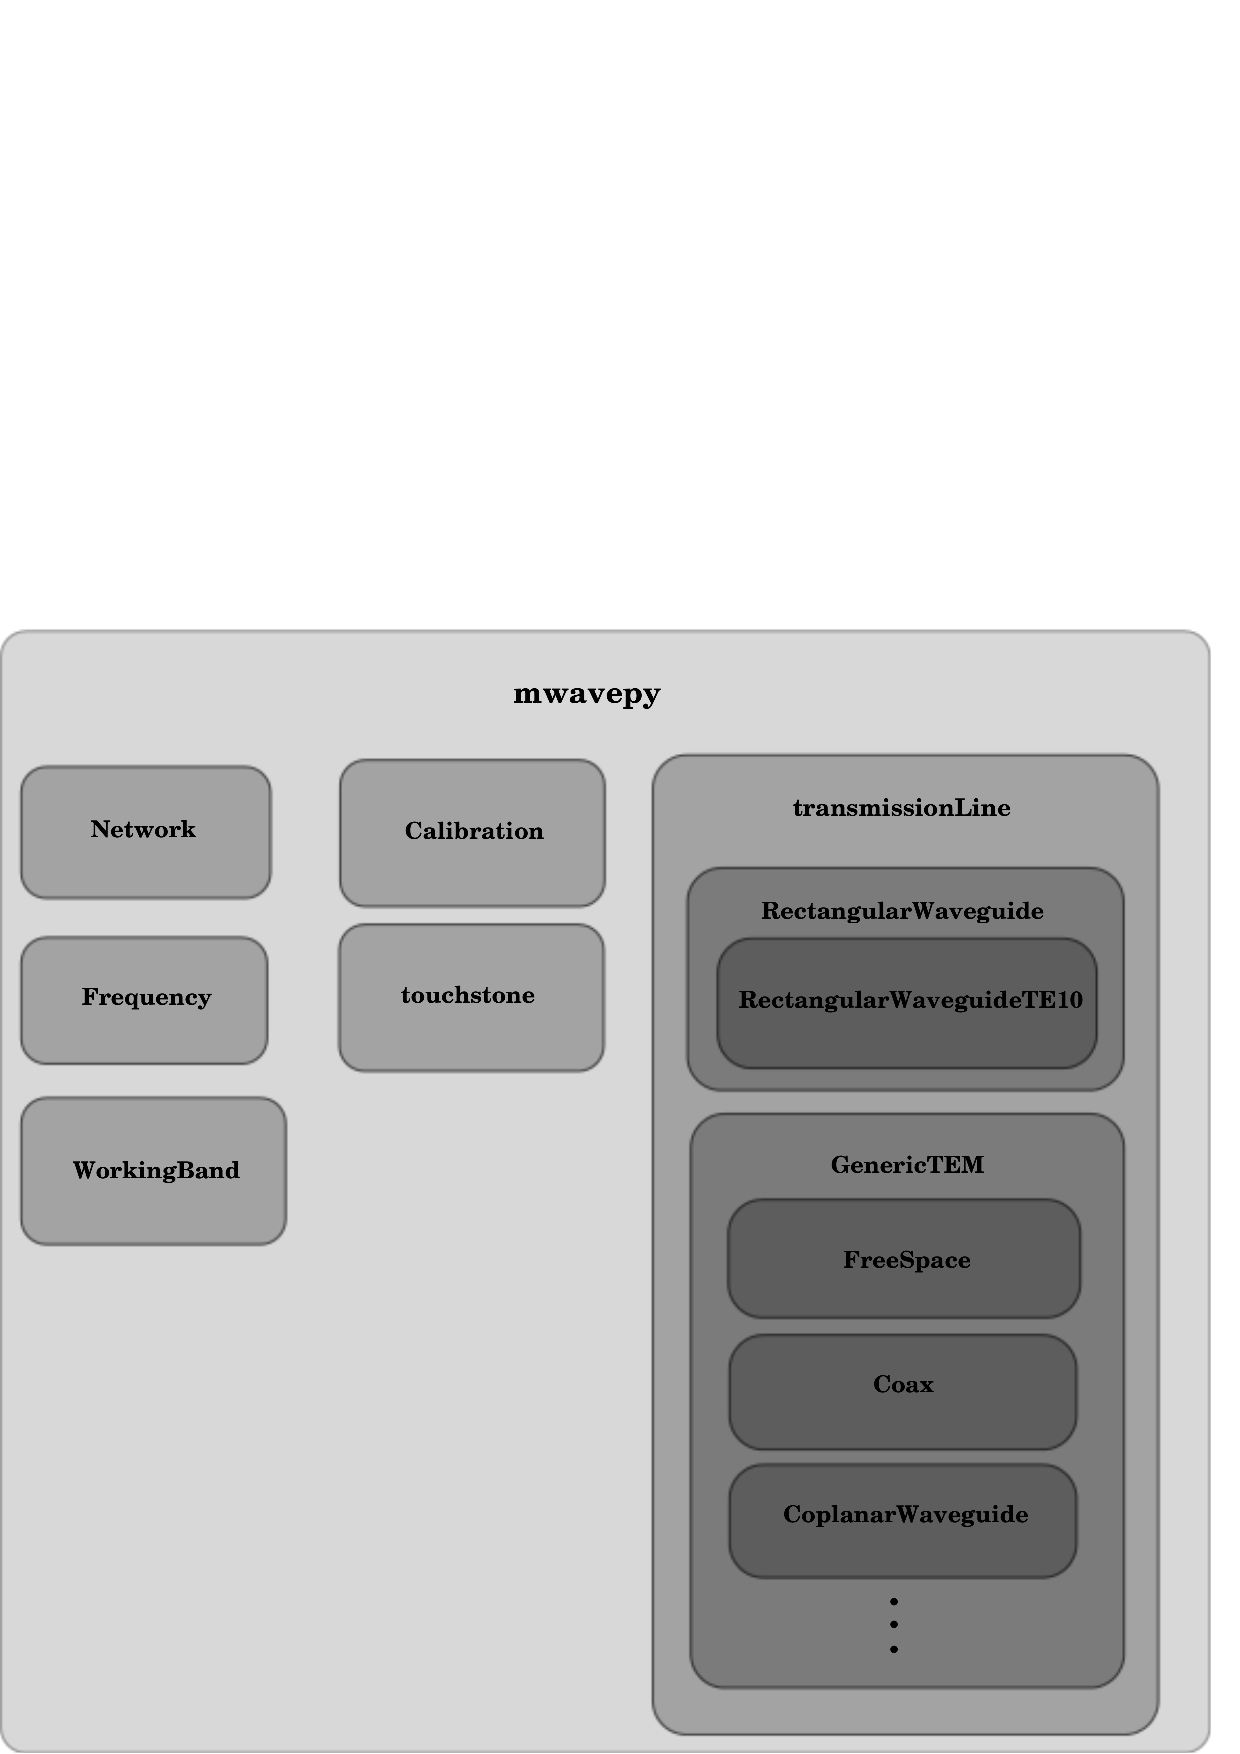
\includegraphics{classInheretanceOutline.pdf}
\end{figure}


\section{Individual Class Architectures}
\label{architecture:individual-class-architectures}\begin{figure}[htbp]
\centering


\includegraphics{images/classOutline.*}
\end{figure}


\subsection{Frequency}
\label{architecture:frequency}
The frequency object was created to make storing and manipulating frequency information easier and more rigid. A major convenience this class provides is the acounting of the frequency vector's unit. Other objects, such as Network, and Calibration require a frequency vector to be meaningful. This vector is commonly referenced when a plot is generated, which one generally doesnt was in units of Hz. If the Frequency object did not exist other objects which require frequency information would have to implement the unit and multiplier bagage.
\begin{figure}[htbp]
\centering


\includegraphics{frequency.pdf}
\end{figure}


\subsection{Network}
\label{architecture:network}\begin{figure}[htbp]
\centering


\includegraphics{network.pdf}
\end{figure}


\subsection{touchstone}
\label{architecture:touchstone}
The standard file format used to store data retrieved from Vector Network Analyzers (VNAs) is the touchstone file format. This file contains all relevent data of a measured network such as frequency info, network parameters (s, y,z, etc), and port impedance.


\subsection{WorkingBand}
\label{architecture:workingband}\begin{figure}[htbp]
\centering

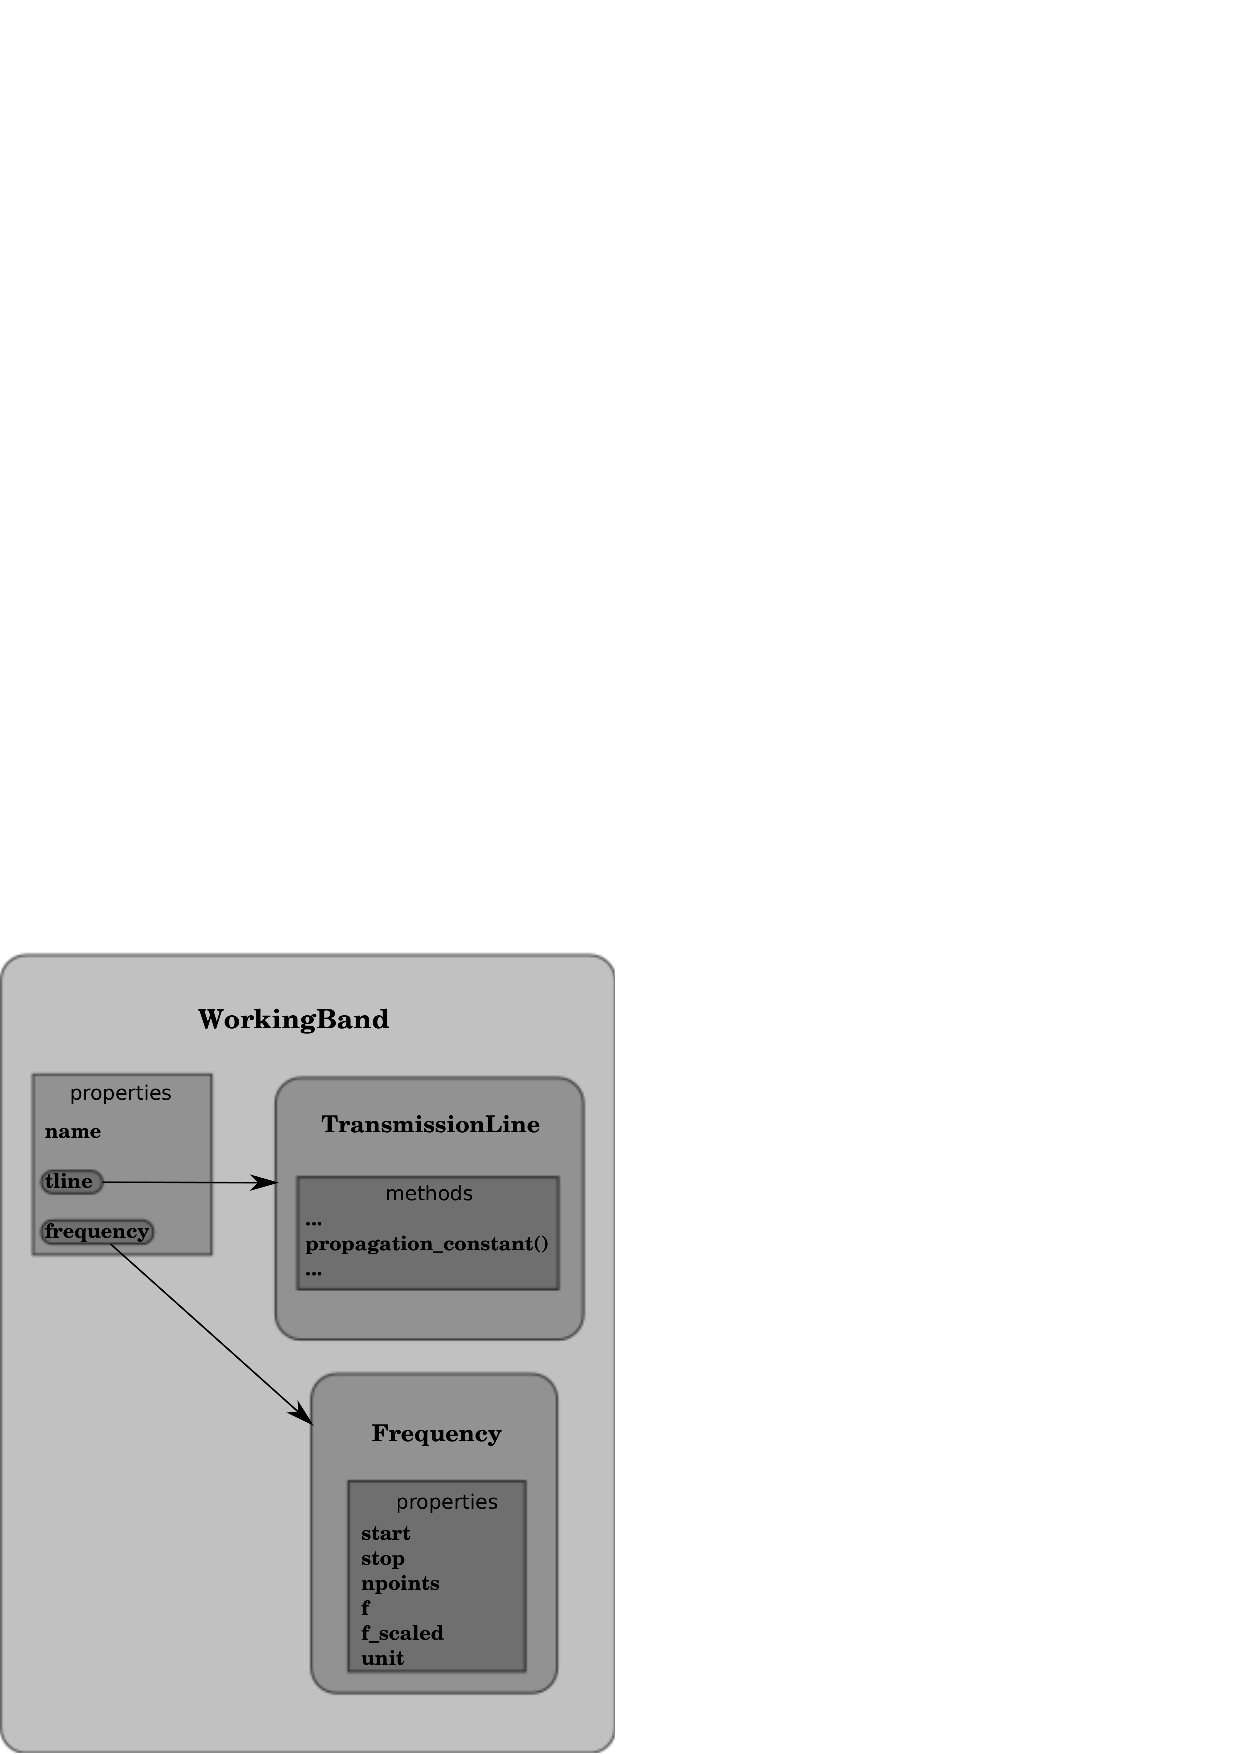
\includegraphics{workingBand.pdf}
\end{figure}


\subsection{Calibration}
\label{architecture:calibration}\begin{figure}[htbp]
\centering

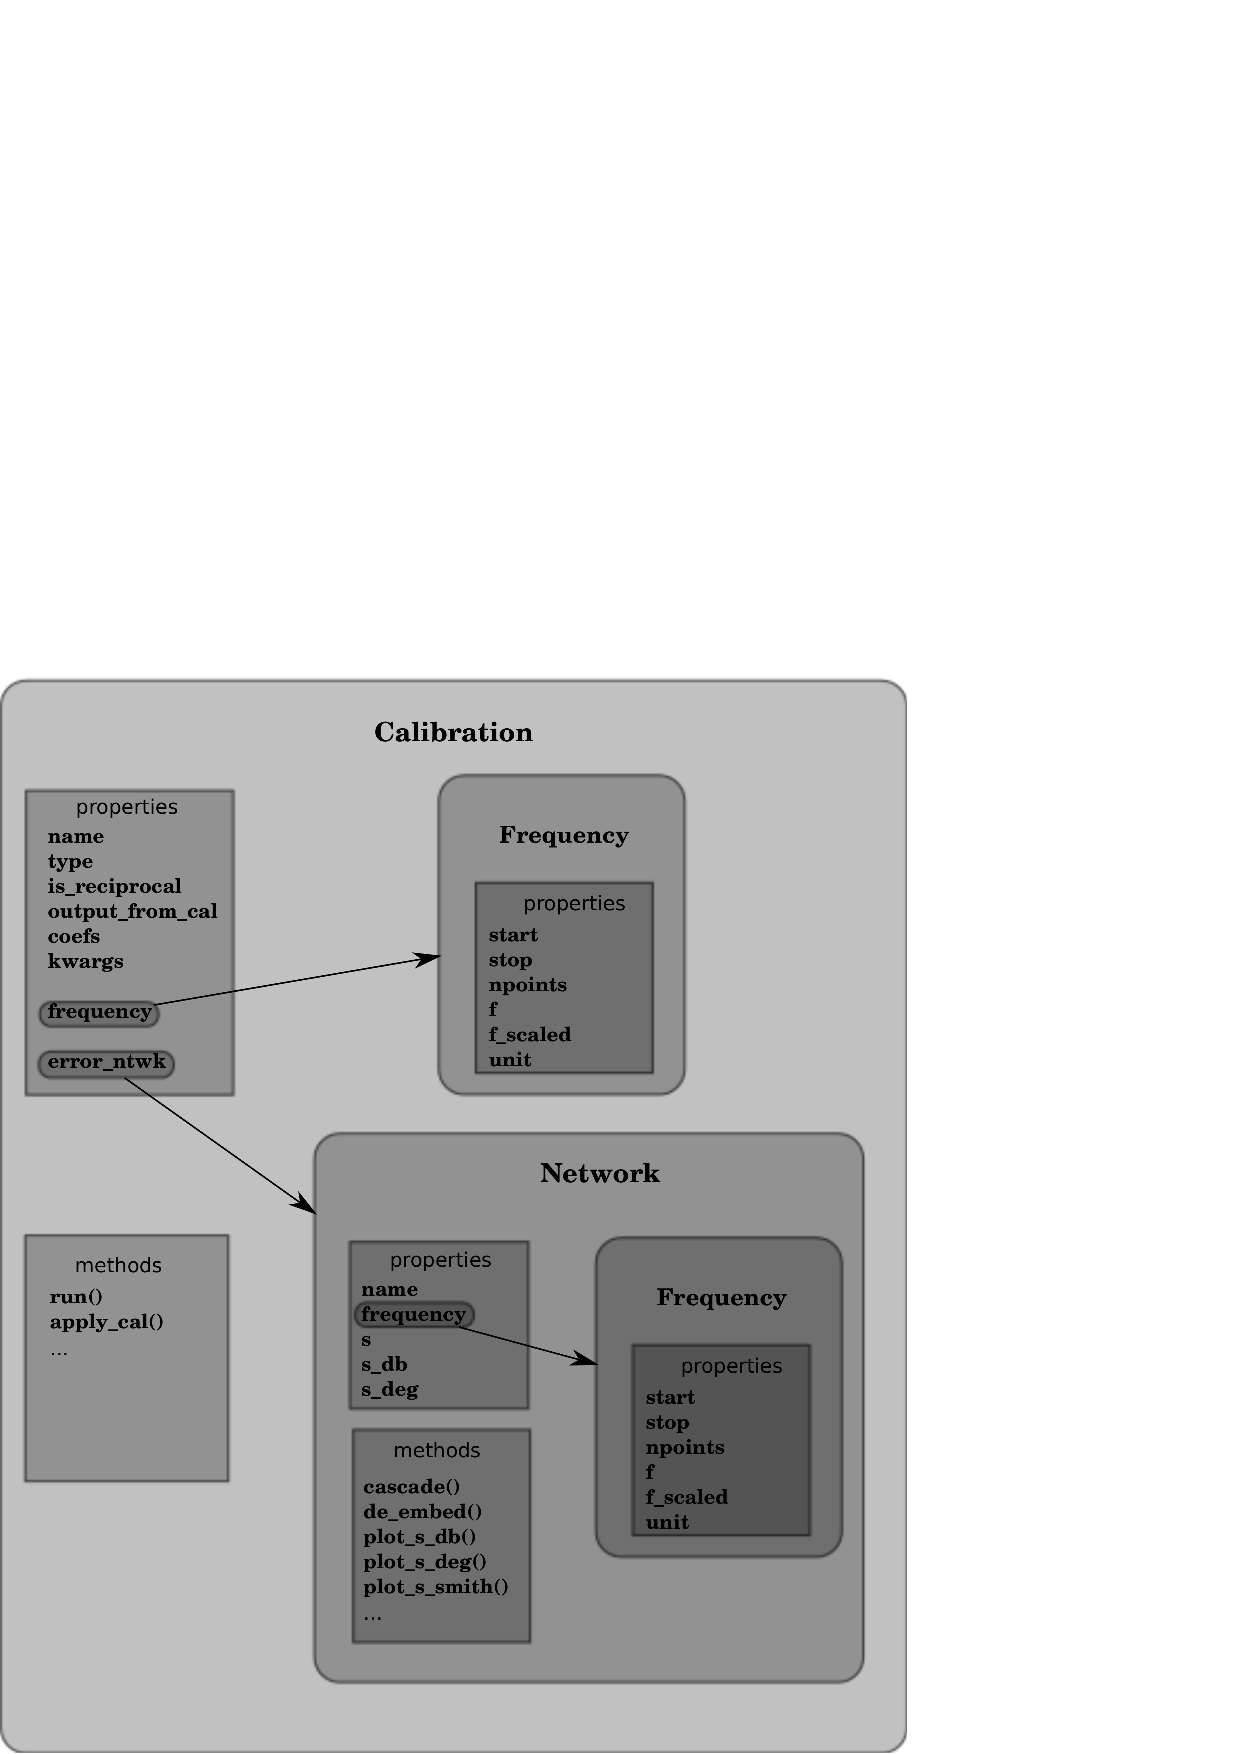
\includegraphics{calibration.pdf}
\end{figure}


\chapter{API}
\label{api:api}\label{api::doc}\label{api:id1}
Major classes


\section{Frequency}
\label{auto_frequency:frequency}\label{auto_frequency::doc}\index{Frequency (class in mwavepy)}

\begin{fulllineitems}
\phantomsection\label{auto_frequency:mwavepy.Frequency}\pysiglinewithargsret{\strong{class }\code{mwavepy.}\bfcode{Frequency}}{\emph{start}, \emph{stop}, \emph{npoints}, \emph{unit='hz'}}{}
represents a frequency band.
\begin{description}
\item[{attributes:}] \leavevmode
start: starting frequency  (in Hz)
stop: stoping frequency  (in Hz)
npoints: number of points, an int
unit: unit which to scale a formated axis, when accesssed. see
\begin{quote}

formattedAxis
\end{quote}

\end{description}

frequently many calcluations are made in a given band , so this class 
is used in other classes so user doesnt have to continually supply 
frequency info.
\index{center (mwavepy.Frequency attribute)}

\begin{fulllineitems}
\phantomsection\label{auto_frequency:mwavepy.Frequency.center}\pysigline{\bfcode{center}}{}
\end{fulllineitems}

\index{f (mwavepy.Frequency attribute)}

\begin{fulllineitems}
\phantomsection\label{auto_frequency:mwavepy.Frequency.f}\pysigline{\bfcode{f}}{}
returns a frequency vector  in Hz

\end{fulllineitems}

\index{f\_scaled (mwavepy.Frequency attribute)}

\begin{fulllineitems}
\phantomsection\label{auto_frequency:mwavepy.Frequency.f_scaled}\pysigline{\bfcode{f\_scaled}}{}
returns a frequency vector in units of self.unit

\end{fulllineitems}

\index{from\_f() (mwavepy.Frequency class method)}

\begin{fulllineitems}
\phantomsection\label{auto_frequency:mwavepy.Frequency.from_f}\pysiglinewithargsret{\strong{classmethod }\bfcode{from\_f}}{\emph{f}}{}
alternative constructor from a frequency vector, in Hz
takes:
\begin{quote}

f: frequency array in Hz
\end{quote}

\end{fulllineitems}

\index{labelXAxis() (mwavepy.Frequency method)}

\begin{fulllineitems}
\phantomsection\label{auto_frequency:mwavepy.Frequency.labelXAxis}\pysiglinewithargsret{\bfcode{labelXAxis}}{\emph{ax=None}}{}
\end{fulllineitems}

\index{multiplier (mwavepy.Frequency attribute)}

\begin{fulllineitems}
\phantomsection\label{auto_frequency:mwavepy.Frequency.multiplier}\pysigline{\bfcode{multiplier}}{}
multiplier for formating axis

\end{fulllineitems}

\index{unit (mwavepy.Frequency attribute)}

\begin{fulllineitems}
\phantomsection\label{auto_frequency:mwavepy.Frequency.unit}\pysigline{\bfcode{unit}}{}
The unit to format the frequency axis in. see formatedAxis

\end{fulllineitems}


\end{fulllineitems}



\section{touchstone}
\label{auto_touchstone::doc}\label{auto_touchstone:touchstone}\index{touchstone (in module mwavepy)}

\begin{fulllineitems}
\phantomsection\label{auto_touchstone:mwavepy.touchstone}\pysigline{\code{mwavepy.}\bfcode{touchstone}}{}
alias of {\hyperref[auto_touchstone:mwavepy.touchstone]{\code{mwavepy.touchstone}}}

\end{fulllineitems}



\section{Network}
\label{auto_network::doc}\label{auto_network:network}\index{Network (class in mwavepy)}

\begin{fulllineitems}
\phantomsection\label{auto_network:mwavepy.Network}\pysiglinewithargsret{\strong{class }\code{mwavepy.}\bfcode{Network}}{\emph{touchstone\_file=None}, \emph{name=None}}{}
Represents a n-port microwave network.
\begin{description}
\item[{the most fundemental properties are:}] \leavevmode\begin{description}
\item[{s: scattering matrix. a kxnxn complex matrix where `n' is number}] \leavevmode
of ports of network.

\end{description}

z0: characteristic impedance
f: frequency vector in Hz. see also frequency, which is a
\begin{quote}

Frequency object (see help on this class for more info)
\end{quote}

\item[{The following operators are defined as follows:}] \leavevmode
`+' : element-wise addition of the s-matrix
`-` : element-wise subtraction of the s-matrix
`*' : element-wise multiplication of the s-matrix
`/' : element-wise division of the s-matrix
`**': cascading of 2-port networks
`//': de-embdeding of one network from the other.

\end{description}

various other network properties are accesable as well as plotting
routines are also defined for convenience,

most properties are derived from the specifications given for
touchstone files.
\index{add\_noise\_polar() (mwavepy.Network method)}

\begin{fulllineitems}
\phantomsection\label{auto_network:mwavepy.Network.add_noise_polar}\pysiglinewithargsret{\bfcode{add\_noise\_polar}}{\emph{mag\_dev}, \emph{phase\_dev}, \emph{**kwargs}}{}
adds a complex zero-mean gaussian white-noise signal of given
standard deviations for magnitude and phase
\begin{description}
\item[{takes:}] \leavevmode
mag\_mag: standard deviation of magnitude
phase\_dev: standard deviation of phase {[}in degrees{]}
n\_ports: number of ports. defualt to 1

\item[{returns:}] \leavevmode
nothing

\end{description}

\end{fulllineitems}

\index{change\_frequency() (mwavepy.Network method)}

\begin{fulllineitems}
\phantomsection\label{auto_network:mwavepy.Network.change_frequency}\pysiglinewithargsret{\bfcode{change\_frequency}}{\emph{new\_frequency}, \emph{**kwargs}}{}
\end{fulllineitems}

\index{f (mwavepy.Network attribute)}

\begin{fulllineitems}
\phantomsection\label{auto_network:mwavepy.Network.f}\pysigline{\bfcode{f}}{}
the frequency vector for the network, in Hz.

\end{fulllineitems}

\index{flip() (mwavepy.Network method)}

\begin{fulllineitems}
\phantomsection\label{auto_network:mwavepy.Network.flip}\pysiglinewithargsret{\bfcode{flip}}{}{}
swaps the ports of a two port

\end{fulllineitems}

\index{frequency (mwavepy.Network attribute)}

\begin{fulllineitems}
\phantomsection\label{auto_network:mwavepy.Network.frequency}\pysigline{\bfcode{frequency}}{}
returns a Frequency object, see  frequency.py

\end{fulllineitems}

\index{interpolate() (mwavepy.Network method)}

\begin{fulllineitems}
\phantomsection\label{auto_network:mwavepy.Network.interpolate}\pysiglinewithargsret{\bfcode{interpolate}}{\emph{new\_frequency}, \emph{**kwargs}}{}
calculates an interpolated network. defualt interpolation type
is linear. see notes about other interpolation types
\begin{description}
\item[{takes:}] \leavevmode
new\_frequency:
{\color{red}\bfseries{}**}kwargs: passed to scipy.interpolate.interp1d initializer.

\item[{returns:}] \leavevmode
result: an interpolated Network

\item[{note:}] \leavevmode\begin{description}
\item[{usefule keyward for  scipy.interpolate.interp1d:}] \leavevmode\begin{description}
\item[{kind}] \leavevmode{[}str or int{]}
Specifies the kind of interpolation as a string (`linear',
`nearest', `zero', `slinear', `quadratic, `cubic') or as an integer
specifying the order of the spline interpolator to use.

\end{description}

\end{description}

\end{description}

\end{fulllineitems}

\index{inv (mwavepy.Network attribute)}

\begin{fulllineitems}
\phantomsection\label{auto_network:mwavepy.Network.inv}\pysigline{\bfcode{inv}}{}
a network representing inverse s-parameters, for de-embeding

\end{fulllineitems}

\index{multiply\_noise() (mwavepy.Network method)}

\begin{fulllineitems}
\phantomsection\label{auto_network:mwavepy.Network.multiply_noise}\pysiglinewithargsret{\bfcode{multiply\_noise}}{\emph{mag\_dev}, \emph{phase\_dev}, \emph{**kwargs}}{}
multiplys a complex bivariate gaussian white-noise signal
of given standard deviations for magnitude and phase.   
magnitude mean is 1, phase mean is 0
\begin{description}
\item[{takes:}] \leavevmode
mag\_dev: standard deviation of magnitude
phase\_dev: standard deviation of phase {[}in degrees{]}
n\_ports: number of ports. defualt to 1

\item[{returns:}] \leavevmode
nothing

\end{description}

\end{fulllineitems}

\index{nudge() (mwavepy.Network method)}

\begin{fulllineitems}
\phantomsection\label{auto_network:mwavepy.Network.nudge}\pysiglinewithargsret{\bfcode{nudge}}{\emph{amount=1e-12}}{}
perturb s-parameters by small amount. this is usefule to work-around
numerical bugs.
takes:
\begin{quote}

amount: amount to add to s parameters
\end{quote}
\begin{description}
\item[{returns:}] \leavevmode
na

\end{description}

\end{fulllineitems}

\index{number\_of\_ports (mwavepy.Network attribute)}

\begin{fulllineitems}
\phantomsection\label{auto_network:mwavepy.Network.number_of_ports}\pysigline{\bfcode{number\_of\_ports}}{}
the number of ports the network has.

\end{fulllineitems}

\index{passivity (mwavepy.Network attribute)}

\begin{fulllineitems}
\phantomsection\label{auto_network:mwavepy.Network.passivity}\pysigline{\bfcode{passivity}}{}~\begin{quote}

passivity metric for a multi-port network. It returns
\end{quote}

a matrix who's diagonals are equal to the total power 
received at all ports, normalized to the power at a single
excitement  port.

mathmatically, this is a test for unitary-ness of the 
s-parameter matrix.
\begin{description}
\item[{for two port this is }] \leavevmode
( {\color{red}\bfseries{}\textbar{}}S11\textbar{}\textasciicircum{}2 + {\color{red}\bfseries{}\textbar{}}S21\textbar{}\textasciicircum{}2, {\color{red}\bfseries{}\textbar{}}S22\textbar{}\textasciicircum{}2+\textbar{}S12\textbar{}\textasciicircum{}2)

\item[{in general it is  }] \leavevmode
S.H * S

\end{description}

where H is conjugate transpose of S, and * is dot product

note:
see more at,
\href{http://en.wikipedia.org/wiki/Scattering\_parameters\#Lossless\_networks}{http://en.wikipedia.org/wiki/Scattering\_parameters\#Lossless\_networks}

\end{fulllineitems}

\index{plot\_polar\_generic() (mwavepy.Network method)}

\begin{fulllineitems}
\phantomsection\label{auto_network:mwavepy.Network.plot_polar_generic}\pysiglinewithargsret{\bfcode{plot\_polar\_generic}}{\emph{attribute\_r}, \emph{attribute\_theta}, \emph{m=0}, \emph{n=0}, \emph{ax=None}, \emph{show\_legend=True}, \emph{**kwargs}}{}
generic plotting function for plotting a Network's attribute
in polar form

takes:

\end{fulllineitems}

\index{plot\_s\_all\_db() (mwavepy.Network method)}

\begin{fulllineitems}
\phantomsection\label{auto_network:mwavepy.Network.plot_s_all_db}\pysiglinewithargsret{\bfcode{plot\_s\_all\_db}}{\emph{ax=None}, \emph{show\_legend=True}, \emph{**kwargs}}{}
plots all s parameters in log magnitude
\begin{description}
\item[{takes:}] \leavevmode\begin{description}
\item[{ax - matplotlib.axes object to plot on, used in case you}] \leavevmode
want to update an existing plot.

\end{description}

show\_legend: boolean, to turn legend show legend of not
{\color{red}\bfseries{}**}kwargs - passed to the matplotlib.plot command

\end{description}

\end{fulllineitems}

\index{plot\_s\_db() (mwavepy.Network method)}

\begin{fulllineitems}
\phantomsection\label{auto_network:mwavepy.Network.plot_s_db}\pysiglinewithargsret{\bfcode{plot\_s\_db}}{\emph{m=None}, \emph{n=None}, \emph{ax=None}, \emph{show\_legend=True}, \emph{**kwargs}}{}
plots the magnitude of the scattering parameter of indecies m, n
in log magnitude
\begin{description}
\item[{takes:}] \leavevmode
m - first index, int
n - second indext, int
ax - matplotlib.axes object to plot on, used in case you
\begin{quote}

want to update an existing plot.
\end{quote}

show\_legend: boolean, to turn legend show legend of not
{\color{red}\bfseries{}**}kwargs - passed to the matplotlib.plot command

\end{description}

\end{fulllineitems}

\index{plot\_s\_deg() (mwavepy.Network method)}

\begin{fulllineitems}
\phantomsection\label{auto_network:mwavepy.Network.plot_s_deg}\pysiglinewithargsret{\bfcode{plot\_s\_deg}}{\emph{m=None}, \emph{n=None}, \emph{ax=None}, \emph{show\_legend=True}, \emph{**kwargs}}{}
plots the phase of a scattering parameter of indecies m, n in
degrees
\begin{description}
\item[{takes:}] \leavevmode
m - first index, int
n - second indext, int
ax - matplotlib.axes object to plot on, used in case you
\begin{quote}

want to update an existing plot.
\end{quote}

show\_legend: boolean, to turn legend show legend of not
{\color{red}\bfseries{}**}kwargs - passed to the matplotlib.plot command

\end{description}

\end{fulllineitems}

\index{plot\_s\_deg\_unwrapped() (mwavepy.Network method)}

\begin{fulllineitems}
\phantomsection\label{auto_network:mwavepy.Network.plot_s_deg_unwrapped}\pysiglinewithargsret{\bfcode{plot\_s\_deg\_unwrapped}}{\emph{m=None}, \emph{n=None}, \emph{ax=None}, \emph{show\_legend=True}, \emph{**kwargs}}{}
plots the phase of a scattering parameter of indecies m, n in
unwrapped degrees
\begin{description}
\item[{takes:}] \leavevmode
m - first index, int
n - second indext, int
ax - matplotlib.axes object to plot on, used in case you
\begin{quote}

want to update an existing plot.
\end{quote}

show\_legend: boolean, to turn legend show legend of not
{\color{red}\bfseries{}**}kwargs - passed to the matplotlib.plot command

\end{description}

\end{fulllineitems}

\index{plot\_s\_mag() (mwavepy.Network method)}

\begin{fulllineitems}
\phantomsection\label{auto_network:mwavepy.Network.plot_s_mag}\pysiglinewithargsret{\bfcode{plot\_s\_mag}}{\emph{m=None}, \emph{n=None}, \emph{ax=None}, \emph{show\_legend=True}, \emph{**kwargs}}{}
plots the magnitude of a scattering parameter of indecies m, n
not in  magnitude
\begin{description}
\item[{takes:}] \leavevmode
m - first index, int
n - second indext, int
ax - matplotlib.axes object to plot on, used in case you
\begin{quote}

want to update an existing plot.
\end{quote}

show\_legend: boolean, to turn legend show legend of not
{\color{red}\bfseries{}**}kwargs - passed to the matplotlib.plot command

\end{description}

\end{fulllineitems}

\index{plot\_s\_polar() (mwavepy.Network method)}

\begin{fulllineitems}
\phantomsection\label{auto_network:mwavepy.Network.plot_s_polar}\pysiglinewithargsret{\bfcode{plot\_s\_polar}}{\emph{m=0}, \emph{n=0}, \emph{ax=None}, \emph{show\_legend=True}, \emph{**kwargs}}{}
plots the scattering parameter of indecies m, n in polar form
\begin{description}
\item[{takes:}] \leavevmode
m - first index, int
n - second indext, int
ax - matplotlib.axes object to plot on, used in case you
\begin{quote}

want to update an existing plot.
\end{quote}

show\_legend: boolean, to turn legend show legend of not
{\color{red}\bfseries{}**}kwargs - passed to the matplotlib.plot command

\end{description}

\end{fulllineitems}

\index{plot\_s\_rad() (mwavepy.Network method)}

\begin{fulllineitems}
\phantomsection\label{auto_network:mwavepy.Network.plot_s_rad}\pysiglinewithargsret{\bfcode{plot\_s\_rad}}{\emph{m=None}, \emph{n=None}, \emph{ax=None}, \emph{show\_legend=True}, \emph{**kwargs}}{}
plots the phase of a scattering parameter of indecies m, n in
radians
\begin{description}
\item[{takes:}] \leavevmode
m - first index, int
n - second indext, int
ax - matplotlib.axes object to plot on, used in case you
\begin{quote}

want to update an existing plot.
\end{quote}

show\_legend: boolean, to turn legend show legend of not
{\color{red}\bfseries{}**}kwargs - passed to the matplotlib.plot command

\end{description}

\end{fulllineitems}

\index{plot\_s\_rad\_unwrapped() (mwavepy.Network method)}

\begin{fulllineitems}
\phantomsection\label{auto_network:mwavepy.Network.plot_s_rad_unwrapped}\pysiglinewithargsret{\bfcode{plot\_s\_rad\_unwrapped}}{\emph{m=None}, \emph{n=None}, \emph{ax=None}, \emph{show\_legend=True}, \emph{**kwargs}}{}
plots the phase of a scattering parameter of indecies m, n in
unwrapped radians
\begin{description}
\item[{takes:}] \leavevmode
m - first index, int
n - second indext, int
ax - matplotlib.axes object to plot on, used in case you
\begin{quote}

want to update an existing plot.
\end{quote}

show\_legend: boolean, to turn legend show legend of not
{\color{red}\bfseries{}**}kwargs - passed to the matplotlib.plot command

\end{description}

\end{fulllineitems}

\index{plot\_s\_smith() (mwavepy.Network method)}

\begin{fulllineitems}
\phantomsection\label{auto_network:mwavepy.Network.plot_s_smith}\pysiglinewithargsret{\bfcode{plot\_s\_smith}}{\emph{m=None}, \emph{n=None}, \emph{r=1}, \emph{ax=None}, \emph{show\_legend=True}, \emph{**kwargs}}{}
plots the scattering parameter of indecies m, n on smith chart
\begin{description}
\item[{takes:}] \leavevmode
m - first index, int
n - second indext, int
r -  radius of smith chart
ax - matplotlib.axes object to plot on, used in case you
\begin{quote}

want to update an existing plot.
\end{quote}

show\_legend: boolean, to turn legend show legend of not
{\color{red}\bfseries{}**}kwargs - passed to the matplotlib.plot command

\end{description}

\end{fulllineitems}

\index{plot\_vs\_frequency\_generic() (mwavepy.Network method)}

\begin{fulllineitems}
\phantomsection\label{auto_network:mwavepy.Network.plot_vs_frequency_generic}\pysiglinewithargsret{\bfcode{plot\_vs\_frequency\_generic}}{\emph{attribute}, \emph{y\_label=None}, \emph{m=None}, \emph{n=None}, \emph{ax=None}, \emph{show\_legend=True}, \emph{**kwargs}}{}
generic plotting function for plotting a Network's attribute
vs frequency.

takes:

\end{fulllineitems}

\index{read\_touchstone() (mwavepy.Network method)}

\begin{fulllineitems}
\phantomsection\label{auto_network:mwavepy.Network.read_touchstone}\pysiglinewithargsret{\bfcode{read\_touchstone}}{\emph{filename}}{}
loads  values from a touchstone file.
\begin{description}
\item[{takes:}] \leavevmode
filename - touchstone file name, string.

\item[{note: }] \leavevmode
ONLY `S' FORMAT SUPORTED AT THE MOMENT 
all work is tone in the touchstone class.

\end{description}

\end{fulllineitems}

\index{s (mwavepy.Network attribute)}

\begin{fulllineitems}
\phantomsection\label{auto_network:mwavepy.Network.s}\pysigline{\bfcode{s}}{}
The scattering parameter matrix.

s-matrix has shape fxnxn, 
where;
\begin{quote}

f is frequency axis and,
n's are port indicies
\end{quote}

\end{fulllineitems}

\index{s11 (mwavepy.Network attribute)}

\begin{fulllineitems}
\phantomsection\label{auto_network:mwavepy.Network.s11}\pysigline{\bfcode{s11}}{}
\end{fulllineitems}

\index{s12 (mwavepy.Network attribute)}

\begin{fulllineitems}
\phantomsection\label{auto_network:mwavepy.Network.s12}\pysigline{\bfcode{s12}}{}
\end{fulllineitems}

\index{s21 (mwavepy.Network attribute)}

\begin{fulllineitems}
\phantomsection\label{auto_network:mwavepy.Network.s21}\pysigline{\bfcode{s21}}{}
\end{fulllineitems}

\index{s22 (mwavepy.Network attribute)}

\begin{fulllineitems}
\phantomsection\label{auto_network:mwavepy.Network.s22}\pysigline{\bfcode{s22}}{}
\end{fulllineitems}

\index{s\_db (mwavepy.Network attribute)}

\begin{fulllineitems}
\phantomsection\label{auto_network:mwavepy.Network.s_db}\pysigline{\bfcode{s\_db}}{}
returns the magnitude of the s-parameters, in dB
\begin{description}
\item[{note:}] \leavevmode\begin{description}
\item[{dB is calculated by }] \leavevmode
20*log10({\color{red}\bfseries{}\textbar{}s\textbar{}})

\end{description}

\end{description}

\end{fulllineitems}

\index{s\_deg (mwavepy.Network attribute)}

\begin{fulllineitems}
\phantomsection\label{auto_network:mwavepy.Network.s_deg}\pysigline{\bfcode{s\_deg}}{}
returns the phase of the s-parameters, in radians

\end{fulllineitems}

\index{s\_deg\_unwrap (mwavepy.Network attribute)}

\begin{fulllineitems}
\phantomsection\label{auto_network:mwavepy.Network.s_deg_unwrap}\pysigline{\bfcode{s\_deg\_unwrap}}{}
returns the unwrapped phase of the s-paramerts, in degrees

\end{fulllineitems}

\index{s\_mag (mwavepy.Network attribute)}

\begin{fulllineitems}
\phantomsection\label{auto_network:mwavepy.Network.s_mag}\pysigline{\bfcode{s\_mag}}{}
returns the magnitude of the s-parameters.

\end{fulllineitems}

\index{s\_rad (mwavepy.Network attribute)}

\begin{fulllineitems}
\phantomsection\label{auto_network:mwavepy.Network.s_rad}\pysigline{\bfcode{s\_rad}}{}
returns the phase of the s-parameters, in radians.

\end{fulllineitems}

\index{s\_rad\_unwrap (mwavepy.Network attribute)}

\begin{fulllineitems}
\phantomsection\label{auto_network:mwavepy.Network.s_rad_unwrap}\pysigline{\bfcode{s\_rad\_unwrap}}{}
returns the unwrapped phase of the s-parameters, in radians.

\end{fulllineitems}

\index{t (mwavepy.Network attribute)}

\begin{fulllineitems}
\phantomsection\label{auto_network:mwavepy.Network.t}\pysigline{\bfcode{t}}{}
returns the t-parameters, which are also known as wave cascading
matrix.

\end{fulllineitems}

\index{write\_touchstone() (mwavepy.Network method)}

\begin{fulllineitems}
\phantomsection\label{auto_network:mwavepy.Network.write_touchstone}\pysiglinewithargsret{\bfcode{write\_touchstone}}{\emph{filename=None}, \emph{dir='./'}}{}
write a touchstone file representing this network.  the only 
format supported at the moment is :
\begin{quote}

HZ S RI
\end{quote}
\begin{description}
\item[{takes: }] \leavevmode\begin{description}
\item[{filename: a string containing filename without }] \leavevmode
extension{[}None{]}. if `None', then will use the network's 
name. if this is empty, then throws an error.

\item[{dir: the directory to save the file in. {[}string{]}. Defaults }] \leavevmode
to `./'

\end{description}

\item[{note:}] \leavevmode
in the future could make possible use of the touchtone 
class, but at the moment this would not provide any benefit 
as it has not {\color{red}\bfseries{}set\_} functions.

\end{description}

\end{fulllineitems}

\index{y (mwavepy.Network attribute)}

\begin{fulllineitems}
\phantomsection\label{auto_network:mwavepy.Network.y}\pysigline{\bfcode{y}}{}
\end{fulllineitems}

\index{z0 (mwavepy.Network attribute)}

\begin{fulllineitems}
\phantomsection\label{auto_network:mwavepy.Network.z0}\pysigline{\bfcode{z0}}{}
the characteristic impedance of the network.

z0 can be may be a number, or numpy.ndarray of shape n or fxn.

\end{fulllineitems}


\end{fulllineitems}



\section{WorkingBand}
\label{auto_workingband::doc}\label{auto_workingband:workingband}\index{WorkingBand (class in mwavepy)}

\begin{fulllineitems}
\phantomsection\label{auto_workingband:mwavepy.WorkingBand}\pysiglinewithargsret{\strong{class }\code{mwavepy.}\bfcode{WorkingBand}}{\emph{tline}, \emph{frequency=None}, \emph{z0=1}}{}~\begin{description}
\item[{A WorkingBand is an high-level object which exists solely to make }] \leavevmode
working with and creation of Networks within the same band,
more concise and convenient.

\item[{A WorkingBand object has three properties: }] \leavevmode
frequency information (Frequency object)
transmission line information   (transmission line object)
character impedance of medium

\item[{the methods of WorkingBand saves the user the hassle of repetitously}] \leavevmode
providing a tline and frequency type for every network creation.

\end{description}

note: frequency and tline classes are copied, so they are passed
by value and not by-reference.
\index{delay\_load() (mwavepy.WorkingBand method)}

\begin{fulllineitems}
\phantomsection\label{auto_workingband:mwavepy.WorkingBand.delay_load}\pysiglinewithargsret{\bfcode{delay\_load}}{\emph{Gamma0}, \emph{d}, \emph{unit='m'}, \emph{**kwargs}}{}
creates a Network for a delayed load transmission line
\begin{description}
\item[{takes:}] \leavevmode
Gamma0: reflection coefficient of load (not in dB)
d: the length (see unit argument) {[}number{]}
unit: string specifying the units of d. possible options are
\begin{quote}

`m': meters, physical length in meters (default)
`deg':degrees, electrical length in degrees
`rad':radians, electrical length in radians
\end{quote}
\begin{description}
\item[{{\color{red}\bfseries{}**}kwargs: key word arguments passed to match(), which is }] \leavevmode
called initially to create a `blank' network. the kwarg
`z0' can be used to create a line of a given impedance

\end{description}

\item[{returns:}] \leavevmode
a 1-port Network class, representing a loaded transmission
line of length d

\end{description}

note: this just calls,
self.line(d,**kwargs) ** self.load(Gamma0, {\color{red}\bfseries{}**}kwargs)

\end{fulllineitems}

\index{delay\_open() (mwavepy.WorkingBand method)}

\begin{fulllineitems}
\phantomsection\label{auto_workingband:mwavepy.WorkingBand.delay_open}\pysiglinewithargsret{\bfcode{delay\_open}}{\emph{d}, \emph{unit='m'}, \emph{**kwargs}}{}
creates a Network for a delayed open transmission line
\begin{description}
\item[{takes:}] \leavevmode
d: the length (see unit argument) {[}number{]}
unit: string specifying the units of d. possible options are
\begin{quote}

`m': meters, physical length in meters (default)
`deg':degrees, electrical length in degrees
`rad':radians, electrical length in radians
\end{quote}
\begin{description}
\item[{{\color{red}\bfseries{}**}kwargs: key word arguments passed to match(), which is }] \leavevmode
called initially to create a `blank' network. the kwarg
`z0' can be used to create a line of a given impedance

\end{description}

\item[{returns:}] \leavevmode
a 1-port Network class, representing a shorted transmission
line of length d

\end{description}

note: this just calls,
self.line(d,**kwargs) ** self.open({\color{red}\bfseries{}**}kwargs)

\end{fulllineitems}

\index{delay\_short() (mwavepy.WorkingBand method)}

\begin{fulllineitems}
\phantomsection\label{auto_workingband:mwavepy.WorkingBand.delay_short}\pysiglinewithargsret{\bfcode{delay\_short}}{\emph{d}, \emph{unit='m'}, \emph{**kwargs}}{}
creates a Network for a delayed short transmission line
\begin{description}
\item[{takes:}] \leavevmode
d: the length (see unit argument) {[}number{]}
unit: string specifying the units of d. possible options are
\begin{quote}

`m': meters, physical length in meters (default)
`deg':degrees, electrical length in degrees
`rad':radians, electrical length in radians
\end{quote}
\begin{description}
\item[{{\color{red}\bfseries{}**}kwargs: key word arguments passed to match(), which is }] \leavevmode
called initially to create a `blank' network. the kwarg
`z0' can be used to create a line of a given impedance

\end{description}

\item[{returns:}] \leavevmode
a 1-port Network class, representing a shorted transmission
line of length d

\end{description}

note: this just calls,
self.line(d,**kwargs) ** self.short({\color{red}\bfseries{}**}kwargs)

\end{fulllineitems}

\index{frequency (mwavepy.WorkingBand attribute)}

\begin{fulllineitems}
\phantomsection\label{auto_workingband:mwavepy.WorkingBand.frequency}\pysigline{\bfcode{frequency}}{}
\end{fulllineitems}

\index{guess\_length\_of\_delay\_short() (mwavepy.WorkingBand method)}

\begin{fulllineitems}
\phantomsection\label{auto_workingband:mwavepy.WorkingBand.guess_length_of_delay_short}\pysiglinewithargsret{\bfcode{guess\_length\_of\_delay\_short}}{\emph{aNtwk}}{}
guess length of physical length of a Delay Short given by aNtwk
\begin{description}
\item[{takes:}] \leavevmode\begin{description}
\item[{aNtwk: a mwavepy.ntwk type . (note: if this is a measurment }] \leavevmode
it needs to be normalized to the reference plane)

\item[{tline: transmission line class of the medium. needed for the }] \leavevmode
calculation of propagation constant

\end{description}

\end{description}

\end{fulllineitems}

\index{impedance\_mismatch() (mwavepy.WorkingBand method)}

\begin{fulllineitems}
\phantomsection\label{auto_workingband:mwavepy.WorkingBand.impedance_mismatch}\pysiglinewithargsret{\bfcode{impedance\_mismatch}}{\emph{z1}, \emph{z2}, \emph{**kwargs}}{}
returns a two-port network for a impedance mis-match
\begin{description}
\item[{takes:}] \leavevmode
z1: complex impedance of port 1 {[} number, list, or 1D ndarray{]}
z2: complex impedance of port 2 {[} number, list, or 1D ndarray{]}
{\color{red}\bfseries{}**}kwargs: passed to mwavepy.Network constructor

\item[{returns:}] \leavevmode
a 2-port network {[}mwavepy.Network{]}

\end{description}

\end{fulllineitems}

\index{line() (mwavepy.WorkingBand method)}

\begin{fulllineitems}
\phantomsection\label{auto_workingband:mwavepy.WorkingBand.line}\pysiglinewithargsret{\bfcode{line}}{\emph{d}, \emph{unit='m'}, \emph{**kwargs}}{}
creates a Network for a section of matched transmission line
\begin{description}
\item[{takes:}] \leavevmode
d: the length (see unit argument) {[}number{]}
unit: string specifying the units of d. possible options are
\begin{quote}

`m': meters, physical length in meters (default)
`deg':degrees, electrical length in degrees
`rad':radians, electrical length in radians
\end{quote}
\begin{description}
\item[{{\color{red}\bfseries{}**}kwargs: key word arguments passed to match(), which is }] \leavevmode
called initially to create a `blank' network. the kwarg
`z0' can be used to create a line of a given impedance

\end{description}

\item[{returns:}] \leavevmode
a 2-port Network class, representing a transmission line of 
length d

\item[{note: }] \leavevmode
the only function called from the tline class is

\end{description}

propagation\_constant(f,d), where f is frequency in Hz and d is
distance in meters. so you can use any class  which provides this
and it  will work .
\begin{description}
\item[{example:}] \leavevmode
wb = WorkingBand(...) \# create a working band object
wb.line(90, `deg', z0=50)

\end{description}

\end{fulllineitems}

\index{load() (mwavepy.WorkingBand method)}

\begin{fulllineitems}
\phantomsection\label{auto_workingband:mwavepy.WorkingBand.load}\pysiglinewithargsret{\bfcode{load}}{\emph{Gamma0}, \emph{nports=1}, \emph{**kwargs}}{}
creates a Network for a Load termianting a transmission line
\begin{description}
\item[{takes:}] \leavevmode
Gamma0: reflection coefficient of load (not in db)
nports: number of ports. creates a short on all ports,
\begin{quote}

default is 1 {[}int{]}
\end{quote}
\begin{description}
\item[{{\color{red}\bfseries{}**}kwargs: key word arguments passed to match(), which is }] \leavevmode
called initially to create a `blank' network

\end{description}

\item[{returns:}] \leavevmode
a 1-port Network class, where  S = Gamma0*ones(...)

\end{description}

\end{fulllineitems}

\index{match() (mwavepy.WorkingBand method)}

\begin{fulllineitems}
\phantomsection\label{auto_workingband:mwavepy.WorkingBand.match}\pysiglinewithargsret{\bfcode{match}}{\emph{nports=1}, \emph{z0=None}, \emph{**kwargs}}{}
creates a Network for a perfect matched transmission line (Gamma0=0)
\begin{description}
\item[{takes:}] \leavevmode
nports: number of ports {[}int{]}
{\color{red}\bfseries{}**}kwargs: key word arguments passed to Network Constructor

\item[{returns:}] \leavevmode
a n-port Network {[}mwavepy.Network{]}

\end{description}

\end{fulllineitems}

\index{open() (mwavepy.WorkingBand method)}

\begin{fulllineitems}
\phantomsection\label{auto_workingband:mwavepy.WorkingBand.open}\pysiglinewithargsret{\bfcode{open}}{\emph{nports=1}, \emph{**kwargs}}{}
creates a Network for a `open' transmission line (Gamma0=1)
\begin{description}
\item[{takes:}] \leavevmode\begin{description}
\item[{nports: number of ports. creates a short on all ports,}] \leavevmode
default is 1 {[}int{]}

\item[{{\color{red}\bfseries{}**}kwargs: key word arguments passed to match(), which is }] \leavevmode
called initially to create a `blank' network

\end{description}

\item[{returns:}] \leavevmode
a n-port Network {[}mwavepy.Network{]}

\end{description}

\end{fulllineitems}

\index{short() (mwavepy.WorkingBand method)}

\begin{fulllineitems}
\phantomsection\label{auto_workingband:mwavepy.WorkingBand.short}\pysiglinewithargsret{\bfcode{short}}{\emph{nports=1}, \emph{**kwargs}}{}
creates a Network for a short  transmission line (Gamma0=-1)
\begin{description}
\item[{takes:}] \leavevmode\begin{description}
\item[{nports: number of ports. creates a short on all ports,}] \leavevmode
default is 1 {[}int{]}

\item[{{\color{red}\bfseries{}**}kwargs: key word arguments passed to match(), which is }] \leavevmode
called initially to create a `blank' network

\end{description}

\item[{returns:}] \leavevmode
a n-port Network {[}mwavepy.Network{]}

\end{description}

\end{fulllineitems}

\index{splitter() (mwavepy.WorkingBand method)}

\begin{fulllineitems}
\phantomsection\label{auto_workingband:mwavepy.WorkingBand.splitter}\pysiglinewithargsret{\bfcode{splitter}}{\emph{nports=3}, \emph{**kwargs}}{}
returns an ideal, lossless n-way splitter.
\begin{description}
\item[{takes:}] \leavevmode
nports: number of ports {[}int{]}
{\color{red}\bfseries{}**}kwargs: key word arguments passed to match(), which is
\begin{quote}

called initially to create a `blank' network.
\end{quote}

\item[{returns:}] \leavevmode
a n-port Network {[}mwavepy.Network{]}

\end{description}

\end{fulllineitems}

\index{tee() (mwavepy.WorkingBand method)}

\begin{fulllineitems}
\phantomsection\label{auto_workingband:mwavepy.WorkingBand.tee}\pysiglinewithargsret{\bfcode{tee}}{\emph{**kwargs}}{}
makes a ideal, lossless tee. (aka three port splitter)
\begin{description}
\item[{takes:}] \leavevmode\begin{description}
\item[{{\color{red}\bfseries{}**}kwargs: key word arguments passed to match(), which is }] \leavevmode
called initially to create a `blank' network.

\end{description}

\item[{returns:}] \leavevmode
a 3-port Network {[}mwavepy.Network{]}

\item[{note:}] \leavevmode
this just calls splitter(3)

\end{description}

\end{fulllineitems}

\index{theta\_2\_d() (mwavepy.WorkingBand method)}

\begin{fulllineitems}
\phantomsection\label{auto_workingband:mwavepy.WorkingBand.theta_2_d}\pysiglinewithargsret{\bfcode{theta\_2\_d}}{\emph{theta}, \emph{deg=True}}{}
converts electrical length to physical distance
\begin{description}
\item[{takes:}] \leavevmode
theta: electrical length, (see deg for unit){[}number{]}
deg: is theta in degrees? {[}boolean{]}

\item[{returns:}] \leavevmode
d: physical distance in meters

\item[{note:}] \leavevmode
this calls the function electrical\_length\_2\_distance which

\end{description}

is provided by transmissionLine.functions.py

\end{fulllineitems}

\index{thru() (mwavepy.WorkingBand method)}

\begin{fulllineitems}
\phantomsection\label{auto_workingband:mwavepy.WorkingBand.thru}\pysiglinewithargsret{\bfcode{thru}}{\emph{**kwargs}}{}
creates a Network for a thru
\begin{description}
\item[{takes:}] \leavevmode\begin{description}
\item[{{\color{red}\bfseries{}**}kwargs: key word arguments passed to match(), which is }] \leavevmode
called initially to create a `blank' network

\end{description}

\item[{returns:}] \leavevmode
a 2-port Network class, representing a thru

\item[{note:}] \leavevmode
this just calls self.line(0)

\end{description}

\end{fulllineitems}

\index{tline (mwavepy.WorkingBand attribute)}

\begin{fulllineitems}
\phantomsection\label{auto_workingband:mwavepy.WorkingBand.tline}\pysigline{\bfcode{tline}}{}
\end{fulllineitems}

\index{two\_port\_reflect() (mwavepy.WorkingBand method)}

\begin{fulllineitems}
\phantomsection\label{auto_workingband:mwavepy.WorkingBand.two_port_reflect}\pysiglinewithargsret{\bfcode{two\_port\_reflect}}{\emph{ntwk1}, \emph{ntwk2}, \emph{**kwargs}}{}
generates a two-port reflective (S21=S12=0) network,from the
responses of 2 one-port networks
\begin{description}
\item[{takes:}] \leavevmode
ntwk1: Network type, seen from port 1
ntwk2: Network type, seen from port 2

\item[{returns:}] \leavevmode
result: two-port reflective Network type

\item[{example:}] \leavevmode
wb.two\_port\_reflect(wb.short(), wb.match())

\end{description}

\end{fulllineitems}

\index{white\_gaussian\_polar() (mwavepy.WorkingBand method)}

\begin{fulllineitems}
\phantomsection\label{auto_workingband:mwavepy.WorkingBand.white_gaussian_polar}\pysiglinewithargsret{\bfcode{white\_gaussian\_polar}}{\emph{phase\_dev}, \emph{mag\_dev}, \emph{n\_ports=1}, \emph{**kwargs}}{}
creates a complex zero-mean gaussian white-noise signal of given
standard deviations for phase and magnitude
\begin{description}
\item[{takes:}] \leavevmode
phase\_mag: standard deviation of magnitude
phase\_dev: standard deviation of phase
n\_ports: number of ports. defualt to 1
{\color{red}\bfseries{}**}kwargs: passed to Network() initializer

\item[{returns:}] \leavevmode
result: Network type

\end{description}

\end{fulllineitems}


\end{fulllineitems}



\section{Calibration}
\label{auto_calibration::doc}\label{auto_calibration:calibration}\index{Calibration (class in mwavepy)}

\begin{fulllineitems}
\phantomsection\label{auto_calibration:mwavepy.Calibration}\pysiglinewithargsret{\strong{class }\code{mwavepy.}\bfcode{Calibration}}{\emph{measured}, \emph{ideals}, \emph{type=None}, \emph{frequency=None}, \emph{is\_reciprocal=False}, \emph{switch\_terms=None}, \emph{name=None}, \emph{**kwargs}}{}
Represents a calibration instance, a class to hold sets
of measurements, ideals, and calibration results.

see init for more information on usage.

note:
all calibration algorithms are in calibrationAlgorithms.py, and are
referenced by the dictionary in this object called
`calibration\_algorihtm\_dict'
\index{Ts (mwavepy.Calibration attribute)}

\begin{fulllineitems}
\phantomsection\label{auto_calibration:mwavepy.Calibration.Ts}\pysigline{\bfcode{Ts}}{}
T-matricies used for de-embeding.

\end{fulllineitems}

\index{apply\_cal() (mwavepy.Calibration method)}

\begin{fulllineitems}
\phantomsection\label{auto_calibration:mwavepy.Calibration.apply_cal}\pysiglinewithargsret{\bfcode{apply\_cal}}{\emph{input\_ntwk}}{}
apply the current calibration to a measurement.
\begin{description}
\item[{takes:}] \leavevmode\begin{description}
\item[{input\_ntwk: the measurement to apply the calibration to, a}] \leavevmode
Network type.

\end{description}

\item[{returns:}] \leavevmode
caled: the calibrated measurement, a Network type.

\end{description}

\end{fulllineitems}

\index{apply\_cal\_to\_all\_in\_dir() (mwavepy.Calibration method)}

\begin{fulllineitems}
\phantomsection\label{auto_calibration:mwavepy.Calibration.apply_cal_to_all_in_dir}\pysiglinewithargsret{\bfcode{apply\_cal\_to\_all\_in\_dir}}{\emph{dir}, \emph{contains=None}, \emph{f\_unit='ghz'}}{}
convience function to apply calibration to an entire directory
of measurements, and return a dictionary of the calibrated
results, optionally the user can `grep' the direction
by using the contains switch.
\begin{description}
\item[{takes:}] \leavevmode
dir: directory of measurements (string)
contains: will only load measurements who's filename contains
\begin{quote}

this string.
\end{quote}
\begin{description}
\item[{f\_unit: frequency unit, to use for all networks. see}] \leavevmode
frequency.Frequency.unit for info.

\end{description}

\item[{returns:}] \leavevmode\begin{description}
\item[{ntwkDict: a dictionary of calibrated measurements, the keys}] \leavevmode
are the filenames.

\end{description}

\end{description}

\end{fulllineitems}

\index{coefs (mwavepy.Calibration attribute)}

\begin{fulllineitems}
\phantomsection\label{auto_calibration:mwavepy.Calibration.coefs}\pysigline{\bfcode{coefs}}{}
coefs: a dictionary holding the calibration coefficients
\begin{description}
\item[{for one port cal's}] \leavevmode
`directivity':e00
`reflection tracking':e01e10
`source match':e11

\item[{for 7-error term two port cal's}] \leavevmode
TBD

\end{description}

\end{fulllineitems}

\index{error\_ntwk (mwavepy.Calibration attribute)}

\begin{fulllineitems}
\phantomsection\label{auto_calibration:mwavepy.Calibration.error_ntwk}\pysigline{\bfcode{error\_ntwk}}{}
a Network type which represents the error network being
calibrated out.

\end{fulllineitems}

\index{frequency (mwavepy.Calibration attribute)}

\begin{fulllineitems}
\phantomsection\label{auto_calibration:mwavepy.Calibration.frequency}\pysigline{\bfcode{frequency}}{}
\end{fulllineitems}

\index{nports (mwavepy.Calibration attribute)}

\begin{fulllineitems}
\phantomsection\label{auto_calibration:mwavepy.Calibration.nports}\pysigline{\bfcode{nports}}{}
the number of ports in the calibration

\end{fulllineitems}

\index{output\_from\_cal (mwavepy.Calibration attribute)}

\begin{fulllineitems}
\phantomsection\label{auto_calibration:mwavepy.Calibration.output_from_cal}\pysigline{\bfcode{output\_from\_cal}}{}
a dictionary holding all of the output from the calibration
algorithm

\end{fulllineitems}

\index{plot\_coefs\_db() (mwavepy.Calibration method)}

\begin{fulllineitems}
\phantomsection\label{auto_calibration:mwavepy.Calibration.plot_coefs_db}\pysiglinewithargsret{\bfcode{plot\_coefs\_db}}{\emph{ax=None}, \emph{show\_legend=True}, \emph{**kwargs}}{}
plot magnitude of the error coeficient dictionary

\end{fulllineitems}

\index{plot\_residuals\_db() (mwavepy.Calibration method)}

\begin{fulllineitems}
\phantomsection\label{auto_calibration:mwavepy.Calibration.plot_residuals_db}\pysiglinewithargsret{\bfcode{plot\_residuals\_db}}{\emph{ax=None}, \emph{show\_legend=True}, \emph{**kwargs}}{}~\begin{description}
\item[{plot magnitude of the resdiues, if calibration is}] \leavevmode
overdetermined

\end{description}

\end{fulllineitems}

\index{residuals (mwavepy.Calibration attribute)}

\begin{fulllineitems}
\phantomsection\label{auto_calibration:mwavepy.Calibration.residuals}\pysigline{\bfcode{residuals}}{}~\begin{description}
\item[{from numpy.lstsq:}] \leavevmode
residues:
the sum of the residues; squared euclidean norm for 
each column vector in b (given ax=b)

\end{description}

\end{fulllineitems}

\index{run() (mwavepy.Calibration method)}

\begin{fulllineitems}
\phantomsection\label{auto_calibration:mwavepy.Calibration.run}\pysiglinewithargsret{\bfcode{run}}{}{}
runs the calibration algorihtm.
\begin{quote}

this is automatically called the
\end{quote}

first time      any dependent property is referenced (like error\_ntwk)
, but only the first time. if you change something and want to
re-run the calibration use this.

\end{fulllineitems}

\index{type (mwavepy.Calibration attribute)}

\begin{fulllineitems}
\phantomsection\label{auto_calibration:mwavepy.Calibration.type}\pysigline{\bfcode{type}}{}
string representing what type of calibration is to be
performed. supported types at the moment are:
\begin{description}
\item[{`one port':     standard one-port cal. if more than}] \leavevmode
2 measurement/ideal pairs are given it will
calculate the least squares solution.

\item[{`one port xds': self-calibration of a unknown-length}] \leavevmode
delay-shorts.

\end{description}

note:
algorithms referenced by  calibration\_algorithm\_dict

\end{fulllineitems}


\end{fulllineitems}



\chapter{Indices and tables}
\label{index:indices-and-tables}\begin{itemize}
\item {} 
\emph{genindex}

\item {} 
\emph{modindex}

\item {} 
\emph{search}

\end{itemize}



\renewcommand{\indexname}{Index}
\printindex
\end{document}
